\documentclass[a4paper, 12pt]{book}
% \documentclass[a4paper, 12pt, draft]{book} % Nalogo preverite tudi z opcijo draft, ki vam bo pokazala, katere vrstice so predolge!



\usepackage[utf8x]{inputenc}   % omogoča uporabo slovenskih črk kodiranih v formatu UTF-8
\usepackage[slovene,english]{babel}    % naloži, med drugim, slovenske delilne vzorce
\usepackage[pdftex]{graphicx}  % omogoča vlaganje slik različnih formatov
\usepackage{fancyhdr}          % poskrbi, na primer, za glave strani
\usepackage{amssymb}           % dodatni simboli
\usepackage{amsmath}           % eqref, npr.
%\usepackage{hyperxmp}
\usepackage[hyphens]{url}  % dodal Solina
\usepackage{comment}       % dodal Solina

\usepackage[pdftex, colorlinks=true,
						citecolor=black, filecolor=black, 
						linkcolor=black, urlcolor=black,
						pagebackref=false, 
						pdfproducer={LaTeX}, pdfcreator={LaTeX}, hidelinks]{hyperref}

\usepackage{color}       % dodal Solina
\usepackage{soul}       % dodal Solina
\usepackage[numbers]{natbib}  % dodal Solina


\usepackage{tikz}
\usepackage{enumitem}
\usepackage{listings}% http://ctan.org/pkg/listings
\lstset{
    basicstyle=\ttfamily,
    mathescape,
    inputencoding = utf8,  % Input encoding
    extendedchars = true,  % Extended ASCII
    literate      =        % Support additional characters
      {Č}{{\v{C}}}1  {č}{{\v{c}}}1  
      {Š}{{\v{S}}}1  {š}{{\v{s}}}1  
      {Ž}{{\v{Z}}}1  {ž}{{\v{z}}}1
}

%%%%%%%%%%%%%%%%%%%%%%%%%%%%%%%%%%%%%%%%
%	DIPLOMA INFO
%%%%%%%%%%%%%%%%%%%%%%%%%%%%%%%%%%%%%%%%
\newcommand{\ttitle}{Inverzije v permutacijah, permutacijski grafi in njihove lastnosti}
\newcommand{\ttitleEn}{Inversions in permutations}
\newcommand{\tsubject}{\ttitle}
\newcommand{\tsubjectEn}{\ttitleEn}
\newcommand{\tauthor}{Luka Uranič}
\newcommand{\tkeywords}{permutacija, inverzija, permutacijski grafi}
\newcommand{\tkeywordsEn}{permutation, inversion, permutation graph}


%%%%%%%%%%%%%%%%%%%%%%%%%%%%%%%%%%%%%%%%
%	HYPERREF SETUP
%%%%%%%%%%%%%%%%%%%%%%%%%%%%%%%%%%%%%%%%
\hypersetup{pdftitle={\ttitle}}
\hypersetup{pdfsubject=\ttitleEn}
\hypersetup{pdfauthor={\tauthor, lu3748@student.uni-lj.is}}
\hypersetup{pdfkeywords=\tkeywordsEn}


 


%%%%%%%%%%%%%%%%%%%%%%%%%%%%%%%%%%%%%%%%
% postavitev strani
%%%%%%%%%%%%%%%%%%%%%%%%%%%%%%%%%%%%%%%%  

\addtolength{\marginparwidth}{-20pt} % robovi za tisk
\addtolength{\oddsidemargin}{40pt}
\addtolength{\evensidemargin}{-40pt}

\renewcommand{\baselinestretch}{1.3} % ustrezen razmik med vrsticami
\setlength{\headheight}{15pt}        % potreben prostor na vrhu
\renewcommand{\chaptermark}[1]%
{\markboth{\MakeUppercase{\thechapter.\ #1}}{}} \renewcommand{\sectionmark}[1]%
{\markright{\MakeUppercase{\thesection.\ #1}}} \renewcommand{\headrulewidth}{0.5pt} \renewcommand{\footrulewidth}{0pt}
\fancyhf{}
\fancyhead[LE,RO]{\sl \thepage} 
%\fancyhead[LO]{\sl \rightmark} \fancyhead[RE]{\sl \leftmark}
\fancyhead[RE]{\sc \tauthor}              % dodal Solina
\fancyhead[LO]{\sc Diplomska naloga}     % dodal Solina


\newcommand{\BibTeX}{{\sc Bib}\TeX}

%%%%%%%%%%%%%%%%%%%%%%%%%%%%%%%%%%%%%%%%
% naslovi
%%%%%%%%%%%%%%%%%%%%%%%%%%%%%%%%%%%%%%%%  


\newcommand{\autfont}{\Large}
\newcommand{\titfont}{\LARGE\bf}
\newcommand{\clearemptydoublepage}{\newpage{\pagestyle{empty}\cleardoublepage}}
\setcounter{tocdepth}{1}	      % globina kazala

%%%%%%%%%%%%%%%%%%%%%%%%%%%%%%%%%%%%%%%%
% konstrukti
%%%%%%%%%%%%%%%%%%%%%%%%%%%%%%%%%%%%%%%%  
\newtheorem{definicija}{Definicija}[chapter]
\newtheorem{lema}{Lema}[chapter]
\newtheorem{izrek}{Izrek}[chapter]
\newtheorem{trditev}{Trditev}[chapter]
\newtheorem{posledica}{Posledica}[chapter]
\newtheorem{domneva}{Domneva}[chapter]
\newenvironment{dokaz}{\emph{Dokaz.}\ }{\hspace{\fill}{$\Box$}}

%%%%%%%%%%%%%%%%%%%%%%%%%%%%%%%%%%%%%%%%%%%%%%%%%%%%%%%%%%%%%%%%%%%%%%%%%%%%%%%
%% PDF-A
%%%%%%%%%%%%%%%%%%%%%%%%%%%%%%%%%%%%%%%%%%%%%%%%%%%%%%%%%%%%%%%%%%%%%%%%%%%%%%%


%%%%%%%%%%%%%%%%%%%%%%%%%%%%%%%%%%%%%%%% 
% define medatata
%%%%%%%%%%%%%%%%%%%%%%%%%%%%%%%%%%%%%%%% 
\def\Title{\ttitle}
\def\Author{\tauthor, lu3748@student.uni-lj.si}
\def\Subject{\ttitleEn}
\def\Keywords{\tkeywordsEn}

%%%%%%%%%%%%%%%%%%%%%%%%%%%%%%%%%%%%%%%% 
% \convertDate converts D:20080419103507+02'00' to 2008-04-19T10:35:07+02:00
%%%%%%%%%%%%%%%%%%%%%%%%%%%%%%%%%%%%%%%% 
\def\convertDate{%
    \getYear
}

{\catcode`\D=12
 \gdef\getYear D:#1#2#3#4{\edef\xYear{#1#2#3#4}\getMonth}
}
\def\getMonth#1#2{\edef\xMonth{#1#2}\getDay}
\def\getDay#1#2{\edef\xDay{#1#2}\getHour}
\def\getHour#1#2{\edef\xHour{#1#2}\getMin}
\def\getMin#1#2{\edef\xMin{#1#2}\getSec}
\def\getSec#1#2{\edef\xSec{#1#2}\getTZh}
\def\getTZh +#1#2{\edef\xTZh{#1#2}\getTZm}
\def\getTZm '#1#2'{%
    \edef\xTZm{#1#2}%
    \edef\convDate{\xYear-\xMonth-\xDay T\xHour:\xMin:\xSec+\xTZh:\xTZm}%
}

\expandafter\convertDate\pdfcreationdate 

%%%%%%%%%%%%%%%%%%%%%%%%%%%%%%%%%%%%%%%%
% get pdftex version string
%%%%%%%%%%%%%%%%%%%%%%%%%%%%%%%%%%%%%%%% 
\newcount\countA
\countA=\pdftexversion
\advance \countA by -100
\def\pdftexVersionStr{pdfTeX-1.\the\countA.\pdftexrevision}


%%%%%%%%%%%%%%%%%%%%%%%%%%%%%%%%%%%%%%%%
% XMP data
%%%%%%%%%%%%%%%%%%%%%%%%%%%%%%%%%%%%%%%%  
\usepackage{xmpincl}
\includexmp{pdfa-1b}

%%%%%%%%%%%%%%%%%%%%%%%%%%%%%%%%%%%%%%%%
% pdfInfo
%%%%%%%%%%%%%%%%%%%%%%%%%%%%%%%%%%%%%%%%  
\pdfinfo{%
    /Title    (\ttitle)
    /Author   (\tauthor, lu3748@student.uni-lj.si)
    /Subject  (\ttitleEn)
    /Keywords (\tkeywordsEn)
    /ModDate  (\pdfcreationdate)
    /Trapped  /False
}


%%%%%%%%%%%%%%%%%%%%%%%%%%%%%%%%%%%%%%%%%%%%%%%%%%%%%%%%%%%%%%%%%%%%%%%%%%%%%%%
%%%%%%%%%%%%%%%%%%%%%%%%%%%%%%%%%%%%%%%%%%%%%%%%%%%%%%%%%%%%%%%%%%%%%%%%%%%%%%%
\let\ab\allowbreak

\begin{document}
\selectlanguage{slovene}
\frontmatter
\setcounter{page}{1} %
\renewcommand{\thepage}{}       % preprecimo težave s številkami strani v kazalu
\newcommand{\sn}[1]{"`#1"'}                    % dodal Solina (slovenski narekovaji)

%%%%%%%%%%%%%%%%%%%%%%%%%%%%%%%%%%%%%%%%
%naslovnica
 \thispagestyle{empty}%
   \begin{center}
    {\large\sc Univerza v Ljubljani\\%
%      Fakulteta za elektrotehniko\\% za študijski program Multimedija
%      Fakulteta za upravo\\% za študijski program Upravna informatika
      Fakulteta za računalništvo in informatiko\\%
      Fakulteta za matematiko in fiziko\\% za študijski program Računalništvo in matematika
     }
    \vskip 10em%
    {\autfont \tauthor\par}%
    {\titfont \ttitle \par}%
    {\vskip 3em \textsc{DIPLOMSKO DELO\\[5mm]         % dodal Solina za ostale študijske programe
%    VISOKOŠOLSKI STROKOVNI ŠTUDIJSKI PROGRAM\\ PRVE STOPNJE\\ RAČUNALNIŠTVO IN INFORMATIKA}\par}%
%    UNIVERZITETNI  ŠTUDIJSKI PROGRAM\\ PRVE STOPNJE\\ RAČUNALNIŠTVO IN INFORMATIKA}\par}%
%    INTERDISCIPLINARNI UNIVERZITETNI\\ ŠTUDIJSKI PROGRAM PRVE STOPNJE\\ MULTIMEDIJA}\par}%
%    INTERDISCIPLINARNI UNIVERZITETNI\\ ŠTUDIJSKI PROGRAM PRVE STOPNJE\\ UPRAVNA INFORMATIKA}\par}%
    INTERDISCIPLINARNI UNIVERZITETNI\\ ŠTUDIJSKI PROGRAM PRVE STOPNJE\\ RAČUNALNIŠTVO IN MATEMATIKA}\par}%
    \vfill\null%
% izberite pravi habilitacijski naziv mentorja!
    {\large \textsc{Mentor}: izr. prof. dr. Polona Oblak\par}%
%    {\large \textsc{Somentor}:  viš. pred./doc./izr. prof./prof. dr.  Martin Krpan \par}%
    {\vskip 2em \large Ljubljana, 2023 \par}%
\end{center}
% prazna stran
%\clearemptydoublepage      % dodal Solina (izjava o licencah itd. se izpiše na hrbtni strani naslovnice)

%%%%%%%%%%%%%%%%%%%%%%%%%%%%%%%%%%%%%%%%
%copyright stran
\thispagestyle{empty}
\vspace*{8cm}

\noindent
{\sc Copyright}. 
Rezultati diplomske naloge so intelektualna lastnina avtorja in matične fakultete Univerze v Ljubljani.
Za objavo in koriščenje rezultatov diplomske naloge je potrebno pisno privoljenje avtorja, fakultete ter mentorja.

\begin{center}
\mbox{}\vfill
\emph{Besedilo je oblikovano z urejevalnikom besedil \LaTeX.}
\end{center}
% prazna stran
\clearemptydoublepage

%%%%%%%%%%%%%%%%%%%%%%%%%%%%%%%%%%%%%%%%
% stran 3 med uvodnimi listi
\thispagestyle{empty}
\
\vfill

\bigskip
\noindent\textbf{Kandidat:} Luka Uranič\\
\noindent\textbf{Naslov:} Inverzije v permutacijah, permutacijski grafi in njihove lastnosti\\
% vstavite ustrezen naziv študijskega programa!
\noindent\textbf{Vrsta naloge:} Diplomska naloga na univerzitetnem programu prve stopnje Računalništvo in matematika \\
% izberite pravi habilitacijski naziv mentorja!
\noindent\textbf{Mentor:}  izr. prof. dr. Polona Oblak\\
% \noindent\textbf{Somentor:} isto kot za mentorja

\bigskip
\noindent\textbf{Opis:}\\
Besedilo teme diplomskega dela študent prepiše iz študijskega informacijskega sistema, kamor ga je vnesel mentor. 
V nekaj stavkih bo opisal, kaj pričakuje od kandidatovega diplomskega dela. 
Kaj so cilji, kakšne metode naj uporabi, morda bo zapisal tudi ključno literaturo.

\bigskip
\noindent\textbf{Title:} Naslov diplome v angleščini

\bigskip
\noindent\textbf{Description:}\\
opis diplome v angleščini

\vfill



\vspace{2cm}

% prazna stran
\clearemptydoublepage

% zahvala
\thispagestyle{empty}\mbox{}\vfill\null\it%
\noindent
Na tem mestu zapišite, komu se zahvaljujete za izdelavo diplomske naloge. Pazite, da ne boste koga pozabili. Utegnil vam bo zameriti. Temu se da izogniti tako, da celotno zahvalo izpustite.
\rm\normalfont

% prazna stran
\clearemptydoublepage

%%%%%%%%%%%%%%%%%%%%%%%%%%%%%%%%%%%%%%%%
% posvetilo, če sama zahvala ne zadošča :-)
% \thispagestyle{empty}\mbox{}{\vskip0.20\textheight}\mbox{}\hfill\begin{minipage}{0.55\textwidth}%
% Svoji dragi Alenčici.
% \normalfont\end{minipage}

% % prazna stran
% \clearemptydoublepage


%%%%%%%%%%%%%%%%%%%%%%%%%%%%%%%%%%%%%%%%
% kazalo
\pagestyle{empty}
\def\thepage{}% preprecimo tezave s stevilkami strani v kazalu
\tableofcontents{}


% prazna stran
\clearemptydoublepage

%%%%%%%%%%%%%%%%%%%%%%%%%%%%%%%%%%%%%%%%
% seznam kratic

\chapter*{Seznam uporabljenih kratic}  % spremenil Solina, da predolge vrstice ne gredo preko desnega roba

\begin{comment}
\begin{tabular}{l|l|l}
  {\bf kratica} & {\bf angleško} & {\bf slovensko} \\ \hline
  % after \\: \hline or \cline{col1-col2} \cline{col3-col4} ...
  {\bf CA} & classification accuracy & klasifikacijska točnost \\
  {\bf DBMS} & database management system & sistem za upravljanje podatkovnih baz \\
  {\bf SVM} & support vector machine & metoda podpornih vektorjev \\
  \dots & \dots & \dots \\
\end{tabular}
\end{comment}

\noindent\begin{tabular}{p{0.1\textwidth}|p{.4\textwidth}|p{.4\textwidth}}    % po potrebi razširi prvo kolono tabele na račun drugih dveh!
  {\bf kratica} & {\bf angleško}                             & {\bf slovensko} \\ \hline
  {\bf CA}      & classification accuracy               & klasifikacijska točnost \\
  {\bf DBMS} & database management system & sistem za upravljanje podatkovnih baz \\
  {\bf SVM}   & support vector machine              & metoda podpornih vektorjev \\
%  \dots & \dots & \dots \\
\end{tabular}


% prazna stran
\clearemptydoublepage

%%%%%%%%%%%%%%%%%%%%%%%%%%%%%%%%%%%%%%%%
% povzetek
\addcontentsline{toc}{chapter}{Povzetek}
\chapter*{Povzetek}

\noindent\textbf{Naslov:} \ttitle
\bigskip

\noindent\textbf{Avtor:} \tauthor
\bigskip

%\noindent\textbf{Povzetek:} 
\noindent V vzorcu je predstavljen postopek priprave diplomskega dela z uporabo okolja \LaTeX. Vaš povzetek mora sicer vsebovati približno 100 besed, ta tukaj je odločno prekratek.
Dober povzetek vključuje: (1) kratek opis obravnavanega problema, (2) kratek opis vašega pristopa za reševanje tega problema in (3) (najbolj uspešen) rezultat ali prispevek magistrske naloge.

\bigskip

\noindent\textbf{Ključne besede:} \tkeywords.
% prazna stran
\clearemptydoublepage

%%%%%%%%%%%%%%%%%%%%%%%%%%%%%%%%%%%%%%%%
% abstract
\selectlanguage{english}
\addcontentsline{toc}{chapter}{Abstract}
\chapter*{Abstract}

\noindent\textbf{Title:} \ttitleEn
\bigskip

\noindent\textbf{Author:} \tauthor
\bigskip

%\noindent\textbf{Abstract:} 
\noindent This sample document presents an approach to typesetting your BSc thesis using \LaTeX. 
A proper abstract should contain around 100 words which makes this one way too short.
\bigskip

\noindent\textbf{Keywords:} \tkeywordsEn.
\selectlanguage{slovene}
% prazna stran
\clearemptydoublepage

%%%%%%%%%%%%%%%%%%%%%%%%%%%%%%%%%%%%%%%%
\mainmatter
\setcounter{page}{1}
\pagestyle{fancy}

% \chapter{ Definicije }
% Naj bo $f: X \rightarrow Y$.\\
% Funkcija f je injektivna: 
% \begin{equation}
%     \label{injektivnost}
%     x_1 \neq x_2 \Rightarrow f(x_1) \neq f(x_2) \Leftrightarrow f(x_1) = f(x_2) \Rightarrow x_1 = x_2
% \end{equation}
% % injektivna : $$ \\
% surjektivna : $\forall y \in Y$ $\exists x \in X: f(x) = y$ \\
% bijektivna: injektivna in surjektivna \\
% $\exists$ injekcija $f: X \rightarrow Y \Rightarrow |X| \leq |Y|$ \\
% $\exists$ surjekcija $f: X \rightarrow Y \Rightarrow |X| \geq |Y|$ \\
% $\exists$ bijekcija $f: X \rightarrow Y \Rightarrow |X| = |Y|$ \\

%%%%%%%%%%%%%%%%%%%%%%%%%%%%%%%%%%%%%%%%%
\chapter{ Notacija, oznake in definicije }
$[n] = \{ 1, 2,..., n\}$. \\
$S_n$ je množico vseh permutacij na množici $[n]$. \\
$id \in S_n$ je permutacija podana s predpisom $id(a) = a$ za $\forall a \in [n]$. \\
$V(G)$ je množica vozlišč grafa $G$. \\
$E(G)$ je množica povezav grafa $G$. \\
$\overline{G}$ je komplement grafa $G$ (nepovezave grafa $G$ so povezave grafa $\overline{G}$). \\
$K_n$ je poln graf na n vozliščih. \\
$\overline{K_n}$ je nepovezan graf na n vozliščih. \\
$P_n$ je pot na n vozliščih. \\
$K_{n, k}$ je dvodelen graf z n vozlišči v eni in k vozlišči v drugi množici. \\
$deg_D^+(x)$ je izhodna stopnja vozlišča $x$ v usmerjenem grafu $D$. \\
$deg_D^-(x)$ je vhodna stopnja vozlišča $x$ v usmerjenem grafu $D$. \\
Premer drevesa je najdaljša pot med dvema vozliščema v grafu. \\
Disjunktna unija grafov pomeni da vzamemo dva grafa in ju združimo v večji graf tako, da ju postavimo drug ob drugega. \\
Določiti smer povezave $vu$ grafa $G$ pomeni spremeniti $vu$ v urejen par $(v, u)$ ali $(u, v)$. \\
Orientacija grafa $G$ je usmerjen graf pridobljen tako da vsaki povezavi grafa $G$ določimo smer. \\

\begin{definicija}[definicija grupe]
    Naj bo A množica. 
    Operacija $\cdot:A \times A \rightarrow A$ vsakemu urejenemu paru elementov iz A priredi natančno določen element iz množice A. 
    Par $(A, \cdot)$ je grupa če velja:
    \begin{enumerate}
        \item $\forall a, b, c \in A: (a \cdot b) \cdot c = a \cdot (b \cdot c)$ (asociativnost)
        \item $\exists e \in A: \forall a \in A: a \cdot e = e \cdot a = a$ (obstoj enote)
        \item $\forall a \in A: \exists a^{-1} \in A: a \cdot a^{-1} = a^{-1} \cdot a = e$ (obstoj inverza)
        
    \end{enumerate}
\end{definicija}
Relacije: $ R\subseteq A\times A, A\neq\emptyset$ \\
R je refleksivna $\Leftrightarrow \forall x\in A: xRx$ \\
R je irefleksivna $\Leftrightarrow \forall x\in A: \neg xRx \Leftrightarrow \overline{R}$ relfeksina \\
R je simetricna $\Leftrightarrow \forall x,y\in A: xRy \Rightarrow yRx \Leftrightarrow R = R^{-1}$ \\
R je asimetricna $\Leftrightarrow \forall x,y\in A: xRy \Rightarrow \neg yRx \Leftrightarrow R \cap R^{-1} = \emptyset$ \\ če asimetricna $\Rightarrow$ irefleksina \\
R je antisimetricna $\Leftrightarrow \forall x,y\in A: xRy \Rightarrow x = y \lor \neg yRx \Leftrightarrow R \cap R^{-1} \subseteq I = \{ (x,x): x \in A\} $ \\
R je tranzitivna $\Leftrightarrow \forall x,y,z\in A: xRy \land yRz \Rightarrow xRz$ \\
R je sovisna $\Leftrightarrow \forall x,y\in A: x \neq y \Rightarrow xRy \lor yRx $ (x in y sta primerljiva)\\
R je strogosovisna $\Leftrightarrow \forall x,y\in A: xRy \lor yRx $\\
Relacije urejenosti: \\
Delna urejenost: R je refleksivna, antisimetricna in tranzitivna [$\subseteq$]\\
Linearna urejenost: R je antisimetricna, strogosovisna, transitivna (refleksivna) [$\leq$]\\ 
Stroga delna urejenost: R je asimetricna in tranzitivna (irefleksivna) [$\subset$] \\
Stroga linearna urejenost: R je asimetricna, sovisna in transitivna [$<$] \\
linearna urejenost $\Rightarrow$ delna urejenost \\
stroga linearna urejenost $\Rightarrow$ stroga delna urejenost \\

%%%%%%%%%%%%%%%%%%%%%%%%%%%%%%%%%%%%%%%%%
\chapter{ Permutacije }

Bijektivni preslikavi $\pi: [n] \rightarrow [n]$ rečemo permutacija (glej sliko \ref
{bijektivna_preslikava_n_n}).
\begin{figure}[h]
    \begin{center}        
        \begin{tikzpicture}[shorten >=1pt,-]
            \tikzstyle{vertex}=[circle,draw=black!0,fill=white!25,minimum size=20pt,inner sep=0pt]
            \foreach \num/\y in {1/1, 2/2, 3/3, 4/4, 5/5}
                \node[vertex] (V-\num) at (0,5-\y) {$\num$};
            \foreach \num/\y in {1/1, 2/2, 3/3, 4/4, 5/5}
                \node[vertex] (VV-\num) at (5, 5-\y) {$\num$};
        
            \foreach \from/\to in {1/3, 2/2, 3/5, 4/1, 5/4}
                \draw[-latex] (V-\from) -- (VV-\to);
        \end{tikzpicture}     
    \end{center}
    \caption{Bijektivna preslikava $[5] \rightarrow [5]$.}
    \label{bijektivna_preslikava_n_n}
\end{figure}

Permutacijo lahko zapišemo na različne načine. 
Zapis permutacije $\pi$ kot vodoravna tabela:
\[
    \pi = \begin{pmatrix}
        1 & 2 & \cdot\cdot\cdot & n \\
        \pi(1) & \pi(2) & \cdot\cdot\cdot & \pi(n)
    \end{pmatrix}
\]
Ker gledamo permutacije na množici $[n]$, ki ima naravno urejenost, lahko zgornjo vrstico izpustimo:
\[
    \pi = (\pi(1), \pi(2), \cdot\cdot\cdot, \pi(n)) = (\pi_1, \pi_2, \cdot\cdot\cdot, \pi_n)
\]
Temu zapisu bomo rekli enovrstični zapis permutacije.
Permutacijo lahko zapišemo tudi kot produkt disjunktnih ciklov:
\[
    \pi = (a_1, a_2, ..., a_i)(b_1, b_2, ..., b_j) \cdot\cdot\cdot (c_1, c_2, ..., c_k)
\]
Ta zapis nam pove, da je 
\[ 
    \pi(a_1) = a_2, \pi(a_2) = a_3, ..., \pi(a_{i-1}) = a_i, \pi(a_i) = a_1
\]
\[
    \pi(b_1) = b_2, \pi(b_2) = b_3, ..., \pi(b_{j-1}) = b_j, \pi(b_j) = b_1    
\]
\[
    \cdot\cdot\cdot
\]
\[
    \pi(c_1) = c_2, \pi(c_2) = c_3, ..., \pi(c_{k-1}) = c_k, \pi(c_k) = c_1
\]

Primer: Naj bo $\pi \in S_5$, $\pi(1) = 3$, $\pi(2) = 5$, $\pi(3) = 1$, $\pi(4) = 4$ in $\pi(5) = 2$. Zapis permutacije $\pi$ kot vodoravna tabela:
\[
    \pi = \begin{pmatrix}
        1 & 2 & 3 & 4 & 5 \\
        3 & 5 & 1 & 4 & 2
    \end{pmatrix}
\]
\[
    \pi = (3, 5, 1, 4, 2) = (3 5 1 4 2) = 35142
\]
Če so vsi elementi permutacije manjši od 10 lahko med številkami vejice izpustimo, vendar ne smemo pozabiti, da ne gre za zapis z disjunktinimi cikli.
Včasih izpustimo tudi oklepaje.
Zapis permutacije $\pi$ kot produkt disjunktnih ciklov:
\[
    \pi = (1 3)(2 5)(4) = (1 3)(2 5)
\]
Ker vemo, da je $\pi \in S_5$ lahko cikel dolžine ena izpustimo.

V nadaljevanju bomo za zapis permutacije uporabljali enovrstični zapis, razen kjer bo navedeno drugače.

\begin{trditev}
    Naj bo $\circ$ kompozitum permutacij. $(S_n, \circ)$ je grupa.
\end{trditev}
\begin{dokaz}
    \begin{enumerate}
        \item Asociativnost: Naj bodo $\pi, \sigma, \tau \in S_n$. Za $\forall i \in [n]$ 
        \[
            ((\pi \circ \sigma) \circ \tau)(i) = (\pi \circ \sigma)(\tau(i)) = \pi(\sigma(\tau(i)))
        \]
        \[
            (\pi \circ (\sigma \circ \tau))(i) = \pi((\sigma \circ \tau)(i)) = \pi(\sigma(\tau(i))) 
        \]
        \item Enota: Za $\forall \pi \in S_n$ in $\forall i \in [n]$ velja:
        \[
            (\pi \circ id)(i) = \pi(id(i)) = \pi(i)
        \]
        \[
            (id \circ \pi)(i) = id(\pi(i)) = \pi(i)
        \]
        \item Inverz: Naj bo $\pi \in S_n$. Ker je $\pi$ bijekcija, $\exists \pi^{-1} \in S_n$.
        \[
            \pi \circ \pi^{-1} = \pi^{-1} \circ \pi = id
        \]
    \end{enumerate}
\end{dokaz}

Grupi $(S_n, \circ)$ rečemo simetrična grupa. Permutacijska grupa je podgrupa simetrične grupe. Po Cayleyevem izreku je vsaka grupa izomorfna neki permutacijski grupi.


%%%%%%%%%%%%%%%%%%%%%%%%%%%%%%%%%%%%%%%%%
\chapter{ Inverzije }

Inverzija permutacije $\sigma = (a_1, a_2,... a_n) \in S_n$ je urejen par $(a_i, a_j)$, kjer je $i < j$ $(\sigma^{-1}(a_i) < \sigma^{-1}(a_j))$ in $a_i > a_j$.

\begin{figure}[h]
    \begin{center}
        \begin{tikzpicture}[shorten >=1pt,-]
            \tikzstyle{vertex}=[circle,draw=black!0,fill=white!25,minimum size=20pt,inner sep=0pt]
            \foreach \num/\y in {1/1, 2/2, 3/3, 4/4}
                \node[vertex] (V-\num) at (0,4-\y) {$\num$};
            \foreach \num/\y in {1/1, 2/2, 3/3, 4/4}
                \node[vertex] (VV-\num) at (4, 4-\y) {$\num$};
        
            \foreach \from/\to in {1/4, 2/2, 3/1, 4/3}
                \draw[latex-latex] (V-\from) -- (VV-\to);

            \draw[-latex] (V-1) .. controls (1, 3.75) and (3, 3.75) .. (VV-1) node[midway, above]{$\sigma$};
            \draw[latex-] (V-4) .. controls (1, -0.5) and (3, -0.5) .. (VV-4) node[midway, above]{$\sigma^{-1}$};

        \end{tikzpicture}
    \end{center}
    \caption{Permutacija $\sigma = (4, 2, 1, 3)$ in njen inverz $\sigma^{-1} = (3, 2, 4, 1)$.}
    \label{permutacija_4213}
\end{figure}

Število inverzij permutacije $\sigma$ je enako številu inverzij permutacije $\sigma^{-1}$. Še več, če ima $\sigma$ inverzije $(a_{i_1}, a_{j_1}), ...., (a_{i_k}, a_{j_k})$, potem ima $\sigma^{-1}$ inverzije $(j_1, i_1), ...., (j_k, i_k)$.

Primer: Naj bo $\sigma = (4, 2, 1, 3)$ kot na sliki \ref{permutacija_4213}, inverzije permutacije $\sigma$ so $(4, 2), (4, 1), (4, 3), (2, 1)$. Pozicije inverzij permutacije $\sigma$ so sledeči pari: $(1, 2), (1, 3), (1, 4), (2, 3)$. Inverz permutacije $\sigma$ je $\sigma^{-1} = (3, 2, 4, 1)$, inverzije permutacije $\sigma^{-1}$ so $(3, 2), \ab (3, 1), (2, 1), (4, 1)$. Opazimo, da so to ravno obrnjeni pari pozicij inverzij permutacije $\sigma$.

Število inverzije je mera, ki nam pove kako daleč je permutacija od urejenega zaporedja $(1, ..., n)$. Urejena permutacija nima inverzij. Največ inverzij ima permutacija $(n, n-1, ..., 1)$ . V tem primeru je vsak par različnih števil $(i, j) \in [n] \times [n], i > j$ v inverziji. Izborov dveh elementov izmed n pa je ravno $\binom{n}{2}$.

Število inverzij je število presečišč v puščičnem diagramu premutacije.

Standardne primerjalne algoritme razvrščanja lahko prilagodimo, tako da izračunamo število inverzij v času $O(n \cdot log(n))$. Primer: Merge sort.

Urediti permutacijo (jo preoblikovali v identično permutacijo) s k inverzijami, je vedno mogoče in zahteva zaporedje k transpozicij sosednjih elementov. Na vsakem koraku izberemo transpozicijo $i$ in $i+1$, če je element na poziciji $i+1$ manjši od elementa na poziciji $i$. Na ta način zmanjšamo število inverzij za 1. To ponavljamo dokler ne pridemo do identične permutacije.

Primer postopka ureditve permutacije $\sigma = (4, 2, 1, 3)$: $\sigma$ ima 4 inverzije. $(ij)$ je ciklični zapis transpozicije elementov $i$ in $j$:
\[
    (4, 2, 1, 3) \overset{(42)}{\rightarrow} (2, 4, 1, 3) \overset{(41)}{\rightarrow} (2, 1, 4, 3) \overset{(43)}{\rightarrow} (2, 1, 3, 4) \overset{(21)}{\rightarrow} (1, 2, 3, 4)
\]

Število permutacij množice [n] s k inverzijami je koeficijent pred $x^k$ v razvoju produkta: 
\[\prod_{m=1}^{n}\sum_{i=0}^{m-1} x^i = 1 (1 + x) (1 + x + x^2) \cdot\cdot\cdot (1 + x + \cdot\cdot\cdot + x^{n-1})\]

Permutacije množice [n] lahko predstavimo tudi, kot celo število $N$, ki je $0 \leq N \leq n!$. Pretvorbo naredimo preko vmesne oblike zaporedja n števil $d_n,d_{n-1},...,d_2,d_1$, kjer je $d_i$ nenegativno celo število manjše od i (pri tem lahko izpustimo $d_1$, saj je vedno $d_1 = 0$). Prvi korak je, da N predstavimo v faktorskem številskem sistemu (angl. factorial number system). Ta sistem ima za števila manjša od $n!$, baze zaporednih števk $(n-1)!,(n-2)!,...,2!,1!$. Drugi korak pa je interpretacija tega zaporedja kot vektor inverzij ali Lehmerjeva koda.

Število zapisano v faktorskem številskem sistemu pretvorimo v desetiški številski sistem tako, da seštejemo produkt vsah števk s pripadajočo bazo. Pretvorbo iz desetiškega v faktorski številski sistem pa naredimo tako, da število zaporedoma delimo z števili $1, 2, 3...$ in si zapisujemo ostanke pri deljenju, dokler ne dobimo 0 kot rezultat deljenja. Zapis števila so ostanki pri deljenju od zadnjega deljenja proti prvemu. Primer pretvorbe: 
\begin{align}
    341010_{!} = 3 \cdot 5! + 4 \cdot 4! + 1 \cdot 3&! + 0 \cdot 2! + 1 \cdot 1! + 0 \cdot 0! = 463_{10} \notag\\
    463 / 1 = 463,&\ ostanek = 0 \notag\\
    463 / 2 = 231,&\ ostanek = 1 \notag\\
    231 / 3 = 77,&\ ostanek = 0 \notag\\
    77 / 4 = 19,&\ ostanek = 1 \notag\\
    19 / 5 = 3,&\ ostanek = 4 \notag\\
    3 / 6 = 0,&\ ostanek = 3 \notag
\end{align}

V Lehmerjevi kodi permutacije $\sigma$, število $d_n$ predstavlja $\sigma_1 - 1 = \sigma(1) - 1$, to je število elementov manjših od $\sigma_1$, ki so v inverziji z $\sigma_1$, število $d_{n-1}$ predstavlja število elementov, ki so manjši od $\sigma_2$ in so v inverziji z $\sigma_2$,... Se pravi $d_{n-i+1}$ predstavlja število elementov, ki so manjši od $\sigma_i$ in so v inverziji z $\sigma_i$.

Vektor inverzij permutacije $\sigma$ je podobn zapis. $d_{n-j+1}$ nam pove koliko je inverzij oblike $(i, j)$, kjer je $j$ manjša vrednost para števil v inverziji.

Obe kodiranji lahko prikažemo z Rothejevim diagramom, kjer pike predstavljajo elemente permutacije, križi pa inverzije permutacije. Lehmerjeva koda nam šteje število križev v vsaki vrstici, vektor inverzij pa šteje število križev v vsakem stolpcu. Poleg tega velja tudi, da je vektor inverzij ravno Lehmerjeva koda inverzne permutacije, in obratno. Primer Rothejevega diagrama je prikazan v tabeli \ref{tbl:rothejev_diagram}.

\begin{table}
    \begin{center}
        \begin{tabular}{ |c|c|c|c|c|c|c|c|c|c|c| } 
        \hline
            $i \setminus \sigma_i$ & 1 & 2 & 3 & 4 & 5 & 6 & 7 & 8 & 9 & Lehmerjeva koda  \\ 
        \hline
            1 & $\times$ & $\times$ & $\times$ & $\times$ & $\times$ & $\cdot$ & & & & $d_9 = 5$  \\ 
        \hline
            2 & $\times$ & $\times$ & $\cdot$ & & & & & & & $d_8 = 2$  \\ 
        \hline
            3 & $\times$ & $\times$ & & $\times$ & $\times$ & & $\times$ & $\cdot$ & & $d_7 = 5$  \\ 
        \hline
            4 & $\cdot$ & & & & & & & & & $d_6 = 0$  \\ 
        \hline
            5 & & $\times$ & & $\cdot$ & & & & & & $d_5 = 1$  \\ 
        \hline
            6 & & $\times$ & & & $\times$ & & $\times$ & & $\cdot$ & $d_4 = 3$  \\ 
        \hline
            7 & & $\times$ & & & $\times$ & & $\cdot$ & & & $d_3 = 2$  \\ 
        \hline
            8 & & $\cdot$ & & & & & & & & $d_2 = 0$  \\ 
        \hline
            9 & & & & & $\cdot$ & & & & & $d_1 = 0$  \\ 
        \hline
            Vektor inverzij & 3 & 6 & 1 & 2 & 4 & 0 & 2 & 0 & 0 &  \\ 
        \hline
        \end{tabular}
    \end{center}
    \caption{ Rothejev diagram za permutacijo $\sigma = (6, 3, 8, 1, 4, 9, 7, 2, 5)$ }
    \label{tbl:rothejev_diagram}
\end{table}

Da bi pretvorili Lehmerjevo kodo $d_n, d_{n-1}, ..., d_1$ v permutacijo, najprej uredimo števila $1, 2, ..., n$ v vrsto. $\sigma_1$ je enak elementu v vrsti, ki je za $d_{n}$ elementi. Nato ta element izbrišemo iz vrste. $\sigma_2$ je enak elemntu v spremenjeni vrsti, ki je za $d_{n-1}$ elemnti. Nato ta element izbrišemo iz vrste in ponovimo postopek za $\sigma_3, ..., \sigma_n$.

Da bi pretvorili tabelo inverzij $d_n, d_{n-1}, ..., d_1$ v permutacijo. Imejmo najprej prazno vrsto. Najprej vzemimo $n$ in ga vstavimo v vrsto za $d_1$ elementi (vedno 0). Nato vzamimo $n-1$ in ga vstavimo v vrsto za $d_{2}$ elementi, ..., vzamemo $1$ in ga vstavimo v vrsto za $d_{n}$ elementi.

Vsota števk v faktorskem zapisu (Lehmerjeva koda ali vektor inverzij) nam pove število inverzij permutacije. Parnost vsote pa nam pove znak permutacije.
\begin{table}
    \begin{center}
        \begin{tabular}{ |c|c|c|c| } 
        \hline
            $\sigma$ & Lehmerjeva koda & Vektor inverzij & Število inverzij \\ 
        \hline
            1234 & 0000 & 0000 & 0 \\ 
        \hline
            1243 & 0010 & 0010 & 1 \\ 
        \hline
            1324 & 0100 & 0100 & 1 \\ 
        \hline
            1342 & 0110 & 0200 & 2 \\ 
        \hline
            1423 & 0200 & 0110 & 2 \\ 
        \hline
            1432 & 0210 & 0210 & 3 \\ 
        \hline
            2134 & 1000 & 1000 & 1 \\ 
        \hline
            2143 & 1010 & 1010 & 2 \\ 
        \hline
            2314 & 1100 & 2000 & 2 \\ 
        \hline
            2341 & 1110 & 3000 & 3 \\ 
        \hline
            2413 & 1200 & 2010 & 3 \\ 
        \hline
            2431 & 1210 & 3010 & 4 \\ 
        \hline
            3124 & 2000 & 1100 & 2 \\ 
        \hline
            3142 & 2010 & 1200 & 3 \\ 
        \hline
            3214 & 2100 & 2100 & 3 \\ 
        \hline
            3241 & 2110 & 3100 & 4 \\ 
        \hline
            3412 & 2200 & 2200 & 4 \\ 
        \hline
            3421 & 2210 & 3200 & 5 \\ 
        \hline
            4123 & 3000 & 1110 & 3 \\ 
        \hline
            4132 & 3010 & 1210 & 4 \\ 
        \hline
            4213 & 3100 & 2110 & 4 \\ 
        \hline
            4231 & 3110 & 3110 & 5 \\ 
        \hline
            4312 & 3200 & 2210 & 5 \\ 
        \hline
            4321 & 3210 & 3210 & 6 \\ 
        \hline
        \end{tabular}
    \end{center}
    \caption{ Permutacije iz $S_4$ z zapisom Lehmerjeve kode in tebele inverzij }
    \label{tbl:permutacije4vektorji}
\end{table}

%%%%%%%%%%%%%%%%%%%%%%%%%%%%%%%%%%%%%%%%%
\chapter{ Permutacijski grafi }

\begin{definicija}
    Naj bo $\sigma \in S_n$. Graf inverzij permutacije $\sigma$, ki ga označimo z $G_{\sigma}$, je neusmerjen graf z $V(G_{\sigma}) = [n]$, kjer je $xy \in E(G_{\sigma})$ natanko tedaj, ko je $(x, y)$ ali $(y, x)$ inverzija permutacije $\sigma$. Vsak graf izomorfen grafu $G_{\sigma}$ za neko permutacijo $\sigma$ imenujemo permutacijski graf.
\end{definicija}

Primer: 
$\sigma = (4, 2, 5, 1, 7, 6, 3) \in S_7$, $V(G_{\sigma}) =[7]$. Množica inverzij $\sigma$ je
$I = \{ (4, 2), (4, 1), (4, 3), (2, 1), (5, 1), (5, 3), (7, 6), (7, 3), (6, 3) \}$
zato je $E(G_{\sigma}) = \{ \{ 4, 2 \}, \{ 4, 1 \}, \{ 4, 3 \}, \{ 2, 1 \}, \{ 5, 1 \}, \{ 5, 3 \}, \{ 7, 6 \}, \{ 7, 3 \}, \{ 6, 3 \} \}$. Graf $G_{\sigma}$ je prikazan na sliki \ref{graf_inverzij}.

\begin{figure}[h]
    \begin{center}        
        \begin{tikzpicture}[shorten >=1pt,-]
            \tikzstyle{vertex}=[circle,draw=black,fill=white!25,minimum size=20pt,inner sep=0pt]
            \foreach \num/\x in {4/1, 2/3, 5/5, 1/7, 7/9, 6/11, 3/13}
                    \node[vertex] (V-\num) at (\x,0) {$\num$};

                \foreach \from/\to in {4/2, 5/1, 7/6, 6/3}
                    \draw (V-\from) -- (V-\to);

                \draw (V-2) .. controls (3.5, 0.75) and (6.5, 0.75) .. (V-1);
                \draw (V-7) .. controls (9.5, 0.75) and (12.5, 0.75) .. (V-3);
                \draw (V-4) .. controls (1.5, 1.5) and (6.5, 1.5) .. (V-1);
                \draw (V-5) .. controls (5.5, 1.5) and (12.5, 1.5) .. (V-3);
                \draw (V-4) .. controls (1, 2.5) and (13, 2.5) .. (V-3);
        \end{tikzpicture}        
    \end{center}
    \caption{Primer grafa inverzij.}
    \label{graf_inverzij}
\end{figure}

Če je graf permutacijski graf, potem lahko veliko problem, ki so NP-polni na poljubnih grafih rešimo v polinomskem času. Na primer: iskanje naječjega podgrafa, ki je poln graf, je ekvivalento iskanju največjega padajočega zaporedja v permutaciji, ki definira permutacijski graf.

\begin{definicija}[Kohezivno zaporedje grafa]
\label{def_kohezivno_zaporedje}
    Naj bo $G$ neusmerjen graf na n vozliščih. 
    Zaporedju vozlišč $l = (v_1, v_2, ..., v_n)$ rečemo kohezivno vozliščno zaporedje grafa $G$ (ali enostavneje kohezivno zaporedje grafa $G$), če sta izpolnjena nasledna pogoja (glej sliko \ref{graf_kohezivno_zaporedje_ab}):
    \begin{enumerate}[label=(\alph*)]
        \item če $i < k < j$ in $v_iv_k$, $v_kv_j \in E(G) \Rightarrow v_iv_j \in E(G)$
        \item če $i < k < j$ in $v_iv_j \in E(G) \Rightarrow v_iv_k \in E(G)$ ali $v_kv_j \in E(G)$
    \end{enumerate}
\end{definicija}

\begin{figure}[h]
    \begin{center}        
        \begin{tikzpicture}[shorten >=1pt,-]
            \tikzstyle{vertex}=[circle,draw=black,fill=white!25,minimum size=20pt,inner sep=0pt]
            \foreach \num/\x in {i/1, k/3, j/5}
                    \node[vertex] (V-\num) at (\x,0) {$v_{\num}$};
            \foreach \num/\x in {i/7, k/9, j/11}
                    \node[vertex] (VV-\num) at (\x,0) {$v_{\num}$};

                \foreach \from/\to in {i/k, k/j}
                    \draw (V-\from) -- (V-\to);
                \foreach \from/\to in {i/k, k/j}
                    \draw[dashed] (VV-\from) -- (VV-\to);


                \draw[dashed] (V-i) .. controls (1.5, 1) and (4.5, 1) .. (V-j);
                \draw (VV-i) .. controls (7.5, 1) and (10.5, 1) .. (VV-j);
        \end{tikzpicture}        
    \end{center}
    \caption{Pogoja za kohezivno zaporedje grafa $G$.}
    \label{graf_kohezivno_zaporedje_ab}
\end{figure}

\begin{lema}
\label{lema0}
    Naj bo $G$ graf. Zaporedje vozlišč $l$ je kohezivno zaporedje grafa $G$ natanko tedaj ko je $l$ kohezivno zaporedje grafa $\overline{G}$ 
\end{lema}
\begin{dokaz}
    $(\Rightarrow)$ Naj bo $l = (v_1, v_2, ..., v_n)$ kohezivno zaporedje grafa $G$. Trdimo, da je $l$ kohezivno zaporedje grafa $\overline{G}$. 
    \begin{enumerate}[label=(\alph*)]
        \item Naj bosta $v_iv_k, v_kv_j \in E(\overline{G})$ tako da $i < k < j$. Potem, po definiciji komplementa $v_iv_k, v_kv_j \notin E(G)$. Če pogoj (b) iz definicije \ref{def_kohezivno_zaporedje} negiramo ($i < k < j$ in $v_iv_k, v_kv_j \notin E(G) \Rightarrow v_iv_j \notin E(G)$) sledi, da $v_iv_j \notin E(G)$. Kar pomeni $v_iv_j \in E(\overline{G})$
        \item Naj bo $v_iv_j \in E(\overline{G})$ tako da $i < j$ in k tako naravno število, da je $i < k < j$. Potem $v_iv_j \notin E(G)$. Če pogoj (a) iz definicije \ref{def_kohezivno_zaporedje} negiramo vidimo, da $v_iv_k \notin E(G)$ ali $v_kv_j \notin E(G)$ (vsaj ena od povezav $v_iv_k, v_kv_j$ ni povezava grafa $G$). Zato sledi, da je $v_iv_k \in E(\overline{G})$ ali $v_kv_j \in E(\overline{G})$. 
    \end{enumerate}
    $(\Leftarrow)$ Obratna smer dokaza sledi iz dejstva, da je $\overline{\overline{G}} = G$.
\end{dokaz}

\begin{izrek}
\label{izrek_sigma_kohezivno_zaporedje}
    Naj bo $\sigma \in S_n$. $\sigma = (\sigma(1), \sigma(2), ..., \sigma(n))$ je kohezivno zaporedje permutacijskega grafa $G_{\sigma}$
\end{izrek}
\begin{dokaz}
    Naj bo $\sigma = (\sigma(1), \sigma(2), ..., \sigma(n)) \in S_n$. Trdimo, da je $\sigma$ kohezivno zaporedje grafa $G_{\sigma}$. 
    \begin{enumerate}[label=(\alph*)]
        \item Če je $i < k < j$ in $\sigma(i)\sigma(k), \sigma(k)\sigma(j) \in E(G_{\sigma})$, potem sta $(\sigma(i),\sigma(k))$ in $(\sigma(k),\sigma(j))$ inverziji permutacije $\sigma$, kar pomeni $\sigma(i) > \sigma(k) > \sigma(j)$. Zato je tudi $(\sigma(i),\sigma(j))$ inverzija permutacije $\sigma$ in $\sigma(i)\sigma(j) \in E(G_{\sigma})$.        

        \item Naj bo $\sigma(i)\sigma(j) \in E(G_{\sigma})$ in k tak da $i < k < j$. Potem je $(\sigma(i),\sigma(j))$ inverzija permutacije $\sigma$ in $\sigma(i) > \sigma(j)$. Če je $\sigma(i) > \sigma(k)$ je $(\sigma(i),\sigma(k))$ inverzija permutacije $\sigma$ in $\sigma(i)\sigma(k) \in E(G_{\sigma})$. Če je $\sigma(k) > \sigma(j)$ je $(\sigma(k), \sigma(j))$ inverzija permutacije $\sigma$ in $\sigma(k)\sigma(j) \in E(G_{\sigma})$. Tako je vsaj ena od povezav $\sigma(i)\sigma(k)$ in $\sigma(k)\sigma(j)$ povezava grafa $G_{\sigma}$.
    \end{enumerate}
\end{dokaz}

Zaporedje vozlišč $(v_1, v_2, ..., v_n)$ je kohezivno zaporedje grafa $G$ natanko tedaj, ko je zaporedje vozlišč $(v_n, v_{n-1}, ..., v_1)$ kohezivno zaporedje grafa $G$.

Za usmerjen graf $D$ rečemo, da je tranzitiven, če je $(x, z)$ usmerjena povezava grafa $D$ kadar sta $(x, y)$ in $(y, z)$ usmerjeni povezavi grafa $D$. 

Polnemu orientiranemu grafu rečemo turnir. Rezultat vozlišča x v turnirju je $s(x) = deg^+(x)$. Rezultatsko zaporedje turnirja je zaporedje rezultatov vozlišč turnirja v nepadajočem vrstnem redu.

\begin{figure}[h]
    \begin{center}        
        \begin{tikzpicture}[shorten >=1pt,-]
            \tikzstyle{vertex}=[circle,draw=black,fill=white!25,minimum size=20pt,inner sep=0pt]
            \foreach \num/\x in {1/1, 2/3}
                    \node[vertex] (V-\num) at (\x,0) {$\num$};
            \foreach \num/\x in {3/1, 4/3}
                    \node[vertex] (V-\num) at (\x,2) {$\num$};
            \foreach \num/\x in {4/5, 3/7, 2/9, 1/11}
                    \node[vertex] (VV-\num) at (\x,0) {$\num$};

                \foreach \from/\to in {1/2, 2/4, 4/3, 1/3, 3/2, 4/1}
                    \draw[-latex] (V-\from) -- (V-\to);
                \foreach \from/\to in {4/3, 3/2, 2/1}
                    \draw[-latex] (VV-\from) -- (VV-\to);

                \draw[-latex] (VV-4) .. controls (5.5, 1) and (8.5, 1) .. (VV-2);
                \draw[-latex] (VV-3) .. controls (7.5, 1) and (10.5, 1) .. (VV-1);
                \draw[-latex] (VV-4) .. controls (5.5, 1.5) and (10.5, 1.5) .. (VV-1);
        \end{tikzpicture}
    \end{center}
    \caption{Levo je turnir, desno je tranzitiven turnir na 4 vozliščih}
    \label{graf_turnirja_in_tranzitivnega_turnirja}
\end{figure}

Obstaja samo en tranzitiven turnir na n vozliščih (do izomorfizma natančno), ki je izomorfen grafu permutacije $\sigma = (n, n-1, ..., 1)$ z usmerjenimi povezavami $x \rightarrow y$, če je $(x, y)$ inverzija. Opazimo tudi, da v tranzitivnem turnirju ni usmerjenih ciklov. 

\begin{izrek}
\label{izrek_tranzitiven_turnir}
    Naj bo T turnir na n vozliščih. Naslednje trditve so ekvivalentne:
    \begin{enumerate}
        \item T je tranzitiven
        \item Za $\forall x,y \in V(T)$ velja, če je $(x, y)$ usmerjena povezava v T potem je $s(x) > s(y)$
        \item Za $\forall x,y \in V(T)$  velja, če je $s(x) > s(y)$ potem je $(x, y)$ usmerjena povezava v $T$
        \item Rezultatsko zaporedje turnirja $T$ je $(0, 1, 2, ..., n-1)$
    \end{enumerate}
\end{izrek}
\begin{dokaz}
    Tranzitiven turnir T na n vozliščih je izomorfen grafu permutacije $\sigma = (n, n-1, ..., 1)$ z usmerjenimi povezavami $x \rightarrow y$, če je $(x, y)$ inverzija. Če uredimo vozlišča od leve proti desni tako kot so v permutaciji $\sigma$ vidimo, da ima vsako vozlišče povezave do vseh vozlišč desno on njega (glej sliko \ref{graf_turnirja_in_tranzitivnega_turnirja}). Iz tega sledijo vse lastnosti iz izreka.
\end{dokaz}

\begin{izrek}
\label{izrek_permutacijski_graf_kohezivno_zaporedje}
    Graf G je permutacijski graf natanko tedaj ko ima kohezivno zaporedje.
\end{izrek}
\begin{dokaz}
    $(\Rightarrow)$ Vsak permutacijski graf $G$ je izomorfen nekemu grafu $G_{\sigma}$ za neko permutacijo $\sigma$. Po izreku \ref{izrek_sigma_kohezivno_zaporedje}, je $\sigma = (\sigma(1), ..., \sigma(n)$ kohezivno zaporedje grafa $G_{\sigma}$. Naj bo f izomorfizem, ki graf $G$ slika v graf $G_{\sigma}$. Potem je $g = f^{-1}$ izomorfizem, ki graf $G_{\sigma}$ slika v graf $G$. Sledi, da je $\pi = (g(\sigma(1)), ..., g(\sigma(n)))$ kohezivno zaporedje grafa $G$, saj je $\sigma$ kohezivno zaporedje grafa $G_{\sigma}$ (glej sliko \ref{graf_izomorfizem_f_k3}).

    \begin{figure}[h]
        \begin{center}        
            \begin{tikzpicture}[shorten >=1pt,-]
                \tikzstyle{vertex}=[circle,draw=black,fill=white!25,minimum size=20pt,inner sep=0pt]
                \foreach \num/\x in {1/1, 3/3.5}
                    \node[vertex] (V-\num) at (\x,0) {$v_\num$};
                    
                    \node[vertex] (V-2) at (2.25, 1.5) {$v_2$};
                
                \foreach \num/\x in {3/6, 2/7.5, 1/9}
                    \node[vertex] (VV-\num) at (\x,0) {$\num$};
    
                    \foreach \from/\to in {1/2, 2/3, 3/1}
                        \draw (V-\from) -- (V-\to);
                    \foreach \from/\to in {3/2, 2/1}
                        \draw (VV-\from) -- (VV-\to);
    
                    \draw (VV-3) .. controls (6.5, 1) and (8.5, 1) .. (VV-1);
            \end{tikzpicture}
        \end{center}
        \caption{Izomorfna grafa $G$ in $G_{\sigma}$}
        \label{graf_izomorfizem_f_k3}
    \end{figure}

    $(\Leftarrow)$ Naj bo $G$ graf s kohezivnim zaporedjem $\pi = (v_1, v_2, ..., v_n)$ (slika \ref{graf_s_kohezivnim_zaporedjem}). 
    \begin{figure}[h]
        \begin{center}
            \begin{tikzpicture}[shorten >=1pt,-]
                \tikzstyle{vertex}=[circle,draw=black,fill=white!25,minimum size=20pt,inner sep=0pt]
                \foreach \num/\x in {1/1, 2/3, 3/5, 4/7}
                        \node[vertex] (V-\num) at (\x,0) {$v_{\num}$};
            
                    \foreach \from/\to in {1/2, 3/4}
                        \draw (V-\from) -- (V-\to);
            
                    \draw (V-1) .. controls (1.5, 1.5) and (6.5, 1.5) .. (V-4);
            \end{tikzpicture}
        \end{center}
        \caption{Graf $G$ s koezivnim zaporedjem $(v_1, v_2, v_3, v_4)$.}
        \label{graf_s_kohezivnim_zaporedjem}
    \end{figure}
    Orientirajmo graf $G$ tako, da vse povezave usmerimo od vozlišča z manjšim indeksom proti vozlišču z večjim indeksom. Če je $i < j$ in $v_iv_j \in E(G)$, tako dobimo $(v_i, v_j)$. Označimo usmerjen graf, ki ga na ta način dobimo z D. Spomnimo se, da je zaradi pogoja $(a)$ iz \ref{def_kohezivno_zaporedje} graf D tranzitiven. Orientirajmo še komplement $\overline{G}$ grafa $G$. Povezave $v_iv_j \in E(\overline{G})$, kjer je $i < j$ usmerimo od večjega indeksa k manjšemu in tako dobimo $(v_j, v_i)$. Označimo dobljeni graf z $\overline{D}$. Zaradi leme \ref{lema0} je $\pi$ kohezivno zaporedje grafa $\overline{G}$. Zato je tudi usmerjen graf $\overline{D}$ tranzitiven. Unija grafov $T = D \cup \overline{D}$ je turnir (orientacija polnega grafa $G \cup \overline{G}$). Glej sliko \ref{graf_tranzitivni_turnir}.
    \begin{figure}[h]
        \begin{center}
            \begin{tikzpicture}[shorten >=1pt,-]
                \tikzstyle{vertex}=[circle,draw=black,fill=white!25,minimum size=20pt,inner sep=0pt]
                \foreach \num/\x in {1/1, 2/3, 3/5, 4/7}
                        \node[vertex] (V-\num) at (\x,0) {$v_{\num}$};
            
                    \foreach \from/\to in {1/2, 3/4}
                        \draw[-latex] (V-\from) -- (V-\to);
                    \draw[-latex] (V-1) .. controls (1.5, 1.5) and (6.5, 1.5) .. (V-4);
                    
                    
                    \draw[dashed, -latex] (V-3) .. controls (4, 0.85) and (2, 0.85) .. (V-1);
                    \draw[dashed, -latex] (V-4) .. controls (6, 0.85) and (4, 0.85) .. (V-2);
                    \draw[dashed, -latex] (V-3) -- (V-2);
            \end{tikzpicture}
        \end{center}
        \caption{ Tranzitiven turnir $T$.}
        \label{graf_tranzitivni_turnir}
    \end{figure}
    Radi bi pokazali, da je T tranzitiven turnir. Naj bosta $(x, y)$ in $(y, z)$ usmerjeni povezavi v grafu $T$. Če bi obe pripadali enemu od $D$ ali $\overline{D}$ bi sledilo, da je $(x, z)$ usmerjena povezava v $T$, saj sta $D$ in $\overline{D}$ tranzitivna. Zato brez škode za splošnost privzamimo, da $(x, y) \in E(D) $ in $(y, z) \in E(\overline{D})$. Če je $(x, z) \in E(D)$ smo končali, saj je potem $(x, z) \in E(T)$. Zato privzamimo da $(x, z) \notin E(D)$. Poglejmo ali je lahko $(z, x) \in E(D)$. Zaradi tranzitivnosti grafa D bi to pomenilo da je tudi $(z, y) \in E(D)$, kar je v protislovju s tem da je  $(y, z) \in E(\overline{D})$. Potem je $(z, x) \in E(\overline{D})$ ali $(x, z) \in E(\overline{D})$. Če je $(z, x) \in E(\overline{D})$, potem zaradi tranzitivnosti $\overline{D}$ in $(y, z), (z, x) \in E(\overline{D})$ sledi, da je $(y, x) \in E(\overline{D})$. To je v protislovju z $(x, y) \in E(D)$. Se pravi nam ostane $(x, z) \in E(\overline{D})$. Sledi, da je $(x, z) \in E(T)$ in T je tranzitiven turnir. Po izreku \ref{izrek_tranzitiven_turnir}, je rezultatsko zaporedje tranzitivnega turnirja $T$ enako $(0, 1, 2, ..., n-1)$. 
    \begin{figure}[h]
        \begin{center}
            \begin{tikzpicture}[shorten >=1pt,-]
                \tikzstyle{vertex}=[circle,draw=black,fill=white!25,minimum size=20pt,inner sep=0pt]
                \foreach \num/\x in {3/1, 1/3, 4/5, 2/7}
                        \node[vertex] (V-\num) at (\x,0) {\num};
            
                    \foreach \from/\to in {3/1, 4/2}
                        \draw (V-\from) -- (V-\to);
                    \draw (V-3) .. controls (1.5, 1.5) and (6.5, 1.5) .. (V-2);
                    
                    
                    % \draw[dotted, -latex] (V-3) .. controls (4, 0.85) and (2, 0.85) .. (V-1);
                    % \draw[dotted, -latex] (V-4) .. controls (6, 0.85) and (4, 0.85) .. (V-2);
                    % \draw[dotted, -latex] (V-3) -- (V-2);
            \end{tikzpicture}
        \end{center}
        \caption{Permutacijski graf $G_\sigma$, $\sigma = (3, 1, 4, 2)$.}
        \label{graf_permutacije3142}
    \end{figure}
    Naj bo $\sigma(i) = 1 + s(v_i)$, kjer je $s(v_i)$ rezultat vozlišča $v_i$ grafa $T$ (glej sliki \ref{graf_tranzitivni_turnir} in \ref{graf_permutacije3142}). Radi bi pokazali, da je $f: v_i \rightarrow 1 + s(v_i) = \sigma(i)$ izomorfizem, ki slika graf $G$ v graf $G_{\sigma}$. Preslikava $f$ je bijektivna, saj imajo vozlišča različne rezultate. Pokazati moramo še, da f ohranja sosenosti vozlišč. Naj bo $v_iv_j \in E(G)$, kjer je $i < j$. Potem je $(v_i, v_j) \in E(D)$. Ker je T tranzitiven turnir, je $s(v_i) > s(v_j)$ (izrek \ref{izrek_tranzitiven_turnir}). Sledi, da je $\sigma(v_i) = 1 + s(v_i) > 1 + s(v_j) = \sigma(v_j)$. Zato je $(\sigma(i), \sigma(j))$ inverzija v $\sigma$ in $f(v_i)f(v_j) \in E(G_{\sigma})$. Obratno, naj bo $xy \in E(G_{\sigma})$. Potem je $(x, y)$ ali $(y, x)$ inverzija v $\sigma$. Privzemimo, da je $(x, y)$ inverzija v $\sigma$. Potem je $x = \sigma(i) = 1 + s(v_i)$ in $y = \sigma(j) = 1 + s(v_j)$, $i < j$. Ker je $(x, y)$ inverzija je $x > y$. Potem je tudi $s(v_i) > s(v_j)$ in $(v_i, v_j) \in E(T)$ (izrek \ref{izrek_tranzitiven_turnir}). Ker je $i < j$ je $(v_i, v_j) \in E(D)$ in posledično $v_iv_j \in E(G)$.
\end{dokaz}


\begin{izrek}
\label{izrek_ekvivalentne_trditve_permutacijski_graf}
    Naj bo $G$ graf. Naslednje trditve so ekvivalentne:
    \begin{enumerate}[label=(\alph*)]
        \item $G$ je permutacijski graf
        \item $\overline{G}$ je permutaciski graf
        \item Vsak induciran podgraf grafa $G$ je permutacijski graf
        \item Vsaka povezana komponenta grafa $G$ je permutacijski graf
    \end{enumerate}
\end{izrek}
\begin{dokaz}
    Ekvivalentnost trditve $(a)$ in $(b)$ sledi iz leme \ref{lema0} in izreka \ref{izrek_permutacijski_graf_kohezivno_zaporedje}. Naj bo $(v_1, v_2, ..., v_n)$ kohezivno zaporedje grafa $G$. Induciran podgraf z vozlišči $\{ v_{i_1}, v_{i_2}, ..., v_{i_k} \}$, kjer $i_1 < i_2 < ... < i_k$, ima kohezivno zaporedje $(v_{i_1}, v_{i_2}, ..., v_{i_k})$ (izpolnjeni sta $(a)$ in $(b)$ iz definicije \ref{def_kohezivno_zaporedje}). Torej induciran podgraf je permutacijski in iz $(a)$ sledi $(c)$. Iz $(c)$ sledi $(d)$, saj je vsaka povezana komponenta induciran podgraf. Pokazati moramo še da iz $(d)$ sledi $(a)$. Naj bo $G$ graf, ki ima povezane komponente $G_1, G_2, ..., G_k$. Povezana komponenta $G_i$ naj ima $n_i$ vozlišč. Ker je vsaka povezana komponenta grafa $G$ permutacijski graf ima vsaka povezana komponenta tudi kohezivno zaporedje. Naj bo $l_i = (v_1^i, v_2^i, ..., v_{n_i}^i)$ kohezivno zaporedje povezane komponente $G_i$. Potem je $l = (l_1, l_2, ..., l_k) = (v_1^1, v_2^1, ..., v_{n_1}^1, v_1^2, v_2^2, ..., v_{n_2}^2, ..., v_1^k, v_2^k, ..., v_{n_k}^k)$ kohezivno zaporedje grafa $G$ in graf $G$ permutacijski. 
\end{dokaz}

Grafi poti $P_n$ in zvezd $K_{1,n}$ so permutacijski grafi saj imajo kohezivno zaporedje (sliki \ref{graf_kohezivnega_zaporedja_pot} in \ref{graf_kohezivnega_zaporedja_zvezda}). Kohezivni zaporedji za pot $P_{13}$ sta permutaciji:
\[
    \sigma_1 = (3, 1, 5, 2, 7, 4, 9, 6, 11, 8, 13, 10, 12)
\] 
in 
\[
    \sigma_2 = (2, 4, 1, 6, 3, 8, 5, 10, 7, 12, 9, 13, 11).
\]
Kohezivno zaporedje za zvezdo $K_{1, n}$ pa je permutacija: 
\[
    \pi = (n+1, 1, 2, ..., n).
\]
\begin{figure}[h]
    \begin{center}        
        \begin{tikzpicture}[shorten >=1pt,-]
            \tikzstyle{vertex}=[circle,draw=black,fill=white!25,minimum size=20pt,inner sep=0pt]
            \foreach \num/\x in {3/1, 1/2, 5/3, 2/4, 7/5, 4/6, 9/7, 6/8, 11/9, 8/10, 10/12}
                    \node[vertex] (V-\num) at (\x,0) {$\num$};
        
                \foreach \from/\to in {3/1, 5/2, 7/4, 9/6, 11/8}
                    \draw (V-\from) -- (V-\to);
        
                \draw (V-3) .. controls (1.5, 0.75) and (3.5, 0.75) .. (V-2);
                \draw (V-5) .. controls (3.5, 0.75) and (5.5, 0.75) .. (V-4);
                \draw (V-7) .. controls (5.5, 0.75) and (7.5, 0.75) .. (V-6);
                \draw (V-9) .. controls (7.5, 0.75) and (9.5, 0.75) .. (V-8);
                \draw (V-11) .. controls (9.5, 0.75) and (11.5, 0.75) .. (V-10);
                % \draw (V-13) .. controls (11.5, 0.75) and (12.5, 0.75) .. (V-12);
                
                \filldraw [black] (11,0) circle (.5pt);
                \filldraw [black] (11.33,0) circle (.5pt);
                % \filldraw [black] (11.5,0) circle (.5pt);
                % \filldraw [black] (12.5,0) circle (.5pt);
                % \filldraw [black] (12.75,0) circle (.5pt);
                % \filldraw [black] (13,0) circle (.5pt);
                
                \filldraw [black] (11,0) circle (.5pt);
                \filldraw [black] (11.6,0.53) circle (.5pt);
                \filldraw [black] (12.2,0.63) circle (.5pt);
                \filldraw [black] (12.8,0.63) circle (.5pt);
                \filldraw [black] (13.4,0.53) circle (.5pt);
                \filldraw [black] (14,0) circle (.5pt);
        \end{tikzpicture}     
    \end{center}
    \caption{Primer kohezivnega zaporedja za pot $P_n$.}
    \label{graf_kohezivnega_zaporedja_pot}
\end{figure}


% \begin{tikzpicture}[shorten >=1pt,-]
%     \tikzstyle{vertex}=[circle,draw=black,fill=white!25,minimum size=20pt,inner sep=0pt]
%     \foreach \num/\x in {2/1, 4/2, 1/3, 6/4, 3/5, 8/6, 5/7, 10/8, 7/9, 12/10, 9/11, 13/12, 11/13}
%             \node[vertex] (V-\num) at (\x,0) {$\num$};

%         \foreach \from/\to in {4/1, 6/3, 8/5, 10/7, 12/9, 13/11}
%             \draw (V-\from) -- (V-\to);

%         \draw (V-2) .. controls (1.5, 0.75) and (2.5, 0.75) .. (V-1);
%         \draw (V-4) .. controls (2.5, 0.75) and (4.5, 0.75) .. (V-3);
%         \draw (V-6) .. controls (4.5, 0.75) and (6.5, 0.75) .. (V-5);
%         \draw (V-8) .. controls (6.5, 0.75) and (8.5, 0.75) .. (V-7);
%         \draw (V-10) .. controls (8.5, 0.75) and (10.5, 0.75) .. (V-9);
%         \draw (V-12) .. controls (10.5, 0.75) and (12.5, 0.75) .. (V-11);
% \end{tikzpicture}

\begin{figure}[h]
    \begin{center}        
        \begin{tikzpicture}[shorten >=1pt,-]
            \tikzstyle{vertex}=[circle,draw=black,fill=white!25,minimum size=28pt,inner sep=0pt]
            \foreach \num/\x in {1/3, 2/5, n/9}
                    \node[vertex] (V-\num) at (\x,0) {$\num$};
                    
                \node[vertex] (V-n+1) at (1,0) {$n\!+\!1$};
                \foreach \from/\to in {n+1/1}
                    \draw (V-\from) -- (V-\to);

                \draw (V-n+1) .. controls (1.5, 0.75) and (4.5, 0.75) .. (V-2);
                \draw (V-n+1) .. controls (1.5, 1.5) and (8.5, 1.5) .. (V-n);

                
                \filldraw [black] (6.5,0) circle (1pt);
                \filldraw [black] (7,0) circle (1pt);
                \filldraw [black] (7.5,0) circle (1pt);
        \end{tikzpicture} 
    \end{center}
    \caption{Primer kohezivnega zaporedja za zvezdo $K_{1, n}$.}
    \label{graf_kohezivnega_zaporedja_zvezda}
\end{figure}

Vidimo, da je pogoj $(a)$ iz definicije kohezivnega zaporedja \ref{def_kohezivno_zaporedje} za poti $P_n$ na prazno izpolnjen, saj ni dveh povezav $v_iv_k$ in $v_kv_j$, kjer so $i < k < j$. Pogoj $(b)$ pa je izpolnjen, saj je vedno ko je $v_iv_j$ povezava in k tak, da $i < k < j$ v grafu ena od povezav $v_iv_k$ ali $v_kv_j$. Podobno je pogoj $(a)$ izpolnjen na prazno za zvezde. Pogoj $(b)$ pa je izpolnjen, saj so vse povezave v grafu oblike $v_{n+1}v_k$ za $k \in \{ 1, 2, ..., n \}$. Zato katerokoli povezavo vzamemo bodo vsa vozlišča med krajiščema izbrane povezave $v_{n+1}v_k$ povezana z vozliščem $v_{n+1}$.

Poti in zvezde so drevesa. Ampak niso vsa drevesa permutacijski grafi. Drevo $K_{1,3}^*$, pridobljeno s subdivizijo vseh povezav zvezde $K_{1,3}$, ni permutacijski graf (slika \ref{graf_subdivizija_k13}).

\begin{figure}[h]
    \begin{center}        
        \begin{tikzpicture}[shorten >=1pt,-]
            \tikzstyle{vertex}=[circle,draw=black,fill=white!25,minimum size=20pt,inner sep=0pt]
                    \node[vertex] (V-0) at (4,4){};
                    \node[vertex] (V-1) at (4,1.75){};
                    \node[vertex] (V-2) at (2,0){};
                    \node[vertex] (V-3) at (6,0){};
        
                \foreach \from/\to in {0/1, 1/2, 1/3}
                    \draw (V-\from) -- (V-\to);
        \end{tikzpicture}\qquad
        \begin{tikzpicture}[shorten >=1pt,-]
            \tikzstyle{vertex}=[circle,draw=black,fill=white!25,minimum size=20pt,inner sep=0pt]
                    \node[vertex] (V-0) at (4,4){};
                    \node[vertex] (V-01) at (4,2.90){};
                    \node[vertex] (V-1) at (4,1.75){};
                    \node[vertex] (V-12) at (3, 0.875){};
                    \node[vertex] (V-2) at (2,0){};
                    \node[vertex] (V-13) at (5,0.875){};
                    \node[vertex] (V-3) at (6,0){};
        
                \foreach \from/\to in {0/01, 12/2, 13/3, 01/1, 1/12, 1/13}
                    \draw (V-\from) -- (V-\to);
        \end{tikzpicture}
    \end{center}
    \caption{Graf $K_{1, 3}$ in $K_{1, 3}^*$.}
    \label{graf_subdivizija_k13}
\end{figure}


\begin{definicija}
    Gosenica je drevo, ki po odstranitvi vseh listov postane pot (slika \ref{graf_gosenice_10_listov}).
\end{definicija}

\begin{figure}[h]
    \begin{center}        
        \begin{tikzpicture}[shorten >=1pt,-]
            \tikzstyle{vertex}=[circle,draw=black,fill=white!25,minimum size=20pt,inner sep=0pt]
                    \node[vertex] (V-0) at (0, 1){};
                    \node[vertex] (V-1) at (2, 1){};
                    \node[vertex] (V-2) at (4, 1){};
                    \node[vertex] (V-3) at (6, 1){};
                    \node[vertex] (V-4) at (8, 1){};
                    \node[vertex] (V-5) at (0, 2){};
                    \node[vertex] (V-6) at (2, 2){};
                    \node[vertex] (V-7) at (1, 2){};
                    \node[vertex] (V-8) at (3, 2){};
                    \node[vertex] (V-9) at (4, 0){};
                    \node[vertex] (V-10) at (5, 0){};
                    \node[vertex] (V-11) at (8, 0){};
                    \node[vertex] (V-12) at (7, 2){};
                    \node[vertex] (V-13) at (8, 2){};
                    \node[vertex] (V-14) at (9, 2){};
        
                \foreach \from/\to in {0/1, 1/2, 2/3, 3/4, 0/5, 1/6, 1/7, 1/8, 2/9, 2/10, 4/11, 4/12, 4/13, 4/14}
                    \draw (V-\from) -- (V-\to);
        \end{tikzpicture}
    \end{center}
    \caption{Graf gosenice z 10 listi.}
    \label{graf_gosenice_10_listov}
\end{figure}


\begin{lema}
    Drevo je gosenica natanko tedaj ko ne vsebuje $K_{1,3}^*$ kot podgraf.
\end{lema}
\begin{dokaz}
    Če je drevo gosenica, potem po odstranitvi vseh listov dobimo pot. Če drevesu $K_{1,3}^*$ odstranimo vse liste ne dobimo poti. Torej tudi če drevo vsebuje $K_{1,3}^*$ kot podgraf, nam po odstranitvi listov ostane graf, ki ni pot. Torej gosenica ne vsebuje podgrafa $K_{1,3}^*$. Če drevo ne vsebuje $K_{1,3}^*$ kot podgraf, potem ima vsako vozlišče največ dva soseda, ki nista lista. Prav tako graf ne vsebuje ciklov, saj je drevo. Po odstranitvi listov drevesa vedno dobimo povezan graf, zato po odstranitvi listov tako dobimo pot. Torej je drevo, ki ne vsebuje podgrafa $K_{1,3}^*$, gosenica.
\end{dokaz}

\begin{figure}[h]
    \begin{center}        
        \begin{tikzpicture}[shorten >=1pt,-]
            \tikzstyle{vertex}=[circle,draw=black,fill=white!25,minimum size=20pt,inner sep=0pt]
            \foreach \num/\x in {l_1/0, 2/1, l_2/2, 1/3, l_3/4, 4/5, l_4/6, 3/7, l_5/8, 6/9, l_6/10, 5/11}
                    \node[vertex] (V-\num) at (\x,0) {$\num$};
        
                \foreach \from/\to in {2/l_2, 4/l_4, 6/l_6}
                    \draw[dashed] (V-\from) -- (V-\to);
        
                \draw[dashed] (V-l_1) .. controls (0.5, 1) and (2.5, 1) .. (V-1);
                \draw[dashed] (V-l_3) .. controls (4.5, 1) and (6.5, 1) .. (V-3);
                \draw[dashed] (V-l_5) .. controls (8.5, 1) and (10.5, 1) .. (V-5);
    
                \draw (V-2) .. controls (1.5, 0.75) and (2.5, 0.75) .. (V-1);
                \draw (V-4) .. controls (5.5, 0.75) and (6.5, 0.75) .. (V-3);
                \draw (V-6) .. controls (9.5, 0.75) and (10.5, 0.75) .. (V-5);
                \draw (V-2) .. controls (1.5, 1.5) and (6.5, 1.5) .. (V-3);
                \draw (V-4) .. controls (5.5, 1.5) and (10.5, 1.5) .. (V-5);
        \end{tikzpicture}
    \end{center}
    \caption{Primer kohezivnega zaporedja gosenice.}
    \label{graf_kohezivnega_zaporedja_gosenice}
\end{figure}
\begin{izrek}
\label{izrek_gosenica_permutacijski_graf}
    Drevo je permutacijski graf natanko tedaj ko je gosenica.
\end{izrek}
\begin{dokaz}
    $(\Rightarrow)$ Če drevo ni gosenica, potem vsebuje $K_{1,3}^*$ kot podgraf. Drevo, ki vsebuje $K_{1,3}^*$ ni permutacijski graf, saj $K_{1,3}^*$ ni permutacijski graf. $(\Leftarrow)$ Potrebno je še pokazati, da je gosenica permutacijski graf. To bomo pokazali tako, da bomo gosenici našli kohezivno zaporedje. Naj bo $C$ gosenica in naj bo $P_n$ pot, ki jo pridobimo iz $C$ tako, da odstranimo liste. Če je $n=1$, potem je $C$ zvezda $K_{1,k}$ za nek $k \geq 0$ ali pa trivialen graf $K_1$. Ker so zvezde in trivialen graf permutacijski grafi, predpostavimo da je $n \geq 2$. Zgradimo kohezivno zaporedje poti $P_n$ kot na primeru od prej. Vse liste lihega vozlišča $i$ na poti vstavimo levo od vozlišče $i+1$ na poti $P_n$. Vse liste sodega vozlišča $i$ na poti vstavimo med vozlišči $i$ in $i-1$ na poti $P_n$. Rezultat je kohezivno zaporedje (slika \ref{graf_kohezivnega_zaporedja_gosenice}). Zato je gosenica C res permutacijski graf.    
\end{dokaz}

\begin{definicija}
    Naj bo $G$ graf z množico vozlišč $V(G) = \{x_1, x_2, ..., x_n\}$ in naj bodo $H_1, H_2, ..., H_n$ poljubni grafi. Kompozicija grafov $H_1, H_2, ..., H_n$ z grafom $G$, označena z $G(H_1, H_2, ..., H_n)$, je graf sestavljen iz disjunktne unije $H_1, H_2, ..., H_n$ in dodanih povezav $a_ib_j$, kjer je $a_i \in V(H_i)$ in $b_j \in V(H_j)$, kadar je $x_ix_j \in E(G)$ (sliki \ref{graf_kompozicija_primer1} in \ref{graf_kompozicija_primer2}). Če je $H_i$ fiksen graf $H$. Potem kompozicijo označimo z $G(H)$. 
\end{definicija}

\begin{figure}[h]
    \begin{center}        
        \begin{tikzpicture}[shorten >=1pt,-]
            \tikzstyle{vertex}=[circle,draw=black,fill=white!25,minimum size=20pt,inner sep=0pt]
                    \node[vertex] (V-0) at (1, 0){$1_{P_2}$};
                    \node[vertex] (V-1) at (0, 1){$2_{P_2}$};
        
                    \node[vertex] (V-2) at (2, 3){$3_{P_3}$};
                    \node[vertex] (V-3) at (3, 3){$4_{P_3}$};
                    \node[vertex] (V-4) at (4, 3){$5_{P_3}$};
                    
                    \node[vertex] (V-5) at (5, 0){$6_{P_1}$};
                    
                \foreach \from/\to in {0/1, 2/3, 3/4, 0/2, 0/3, 0/4, 1/2, 1/3, 1/4, 2/5, 3/5, 4/5}
                    \draw (V-\from) -- (V-\to);
        \end{tikzpicture}
    \end{center}
    \caption{Graf $P_3(P_2, P_3, P_1)$.}
    \label{graf_kompozicija_primer1}
\end{figure}

Vsota grafov L in M, označena z $L + M$, je sestavljena iz disjunktne unije grafov L in M in dodanih povezav $ab$, kjer $a \in V(L)$ in $b \in V(M)$. Se pravi, kompozicija $G(H_1, H_2, ..., H_n)$ je sestavljena iz disjunktne unije grafov $H_i$ in potem iz vsote $H_i + H_j$ za vsak pripadajočo povezavo $x_ix_j \in E(G)$.

\begin{izrek}
\label{izrek_konstrukcija_permutacijskega_grafa}
    Naj bo G graf z n vozlišči in naj bodo $H_1, H_2, ..., H_n$ poljubni grafi. Potem je $G(H_1, H_2, ..., H_n)$ permutacijski graf natanko tedaj ko so $G, H_1, H_2, ..., H_n$ permutacijski grafi.
\end{izrek}
\begin{dokaz}
    $(\Rightarrow)$ Privzamimo, da je $G(H_1, H_2, ..., H_n)$ permutacijski graf. Ker so $H_1, H_2, ..., H_n$ inducirani podgrafi grafa $G(H_1, H_2, ..., H_n)$, so permutacijski grafi po izreku \ref{izrek_ekvivalentne_trditve_permutacijski_graf}. Prav tako lahko vzamemo eno vozlišče iz vsakega od grafov $H_i$ in ga označimo z $x_i$. Tako dobimo induciran podgraf izomorfen grafu G. To pomeni, da je tudi G permutacijski. $(\Leftarrow)$ Obratno privzamemo, da so $G, H_1, H_2, ..., H_n$ permutacijski grafi. Potem je $(v_1, v_2, ..., v_n)$ kohezivno zaporedje grafa G. Grafe $H_1, H_2, ..., H_n$ ustrezno preimenujemo tako da je graf, ki pripada vozlišču $v_1$ poimenovan $H_1$, graf, ki pripada vozlišču $v_2$ poimenovan $H_2$, ..., graf, ki pripada vozlišču $v_n$ poimenovan $H_n$. Z $n_i$ označimo število vozlišč grafa $H_i$. Potem ima graf $H_i$ kohezivno zaporedje $l_i = (x_1^i, x_2^i, ..., x_{n_i}^i)$. Se pravi je $l = (l_1, l_2, ..., l_n) = (x_1^1, x_2^1, ..., x_{n_1}^1, x_1^2, x_2^2, ..., x_{n_2}^2, ..., x_1^n, x_2^n, ..., x_{n_n}^n)$ kohezivno zaporedje grafa $G(H_1, H_2, ..., H_n)$ in $G(H_1, H_2, ..., H_n)$ je permutacijski graf.
\end{dokaz}

Izrek \ref{izrek_konstrukcija_permutacijskega_grafa} nam podaja enostaven način konstrukcije permutacijskih grafov. Naj bo $G$ polni graf $K3$. Poglejmo si kompozicijo $K_3(P_2, C_3, P_1)$ (slika \ref{graf_kompozicija_primer2}). Ker so $K_3, P_2, C_3, P_1$ polni grafi dobimo polni graf $K_6$.

\begin{figure}[h]
    \begin{center}        
        \begin{tikzpicture}[shorten >=1pt,-]
            \tikzstyle{vertex}=[circle,draw=black,fill=white!25,minimum size=20pt,inner sep=0pt]
                    \node[vertex] (V-0) at (1.5, 0){$1_{P_2}$};
                    \node[vertex] (V-1) at (-0.5, 1){$2_{P_2}$};
        
                    \node[vertex] (V-2) at (2, 2){$3_{C_3}$};
                    \node[vertex] (V-3) at (3, 3){$4_{C_3}$};
                    \node[vertex] (V-4) at (4, 2){$5_{C_3}$};
                    
                    \node[vertex] (V-5) at (4.5, 0){$6_{P_1}$};
                    
                \foreach \from/\to in {0/1, 2/3, 3/4, 4/2, 0/2, 0/3, 0/4, 1/2, 1/3, 1/4, 2/5, 3/5, 4/5, 0/5, 1/5}
                    \draw (V-\from) -- (V-\to);
        \end{tikzpicture}
    \end{center}
    \caption{Graf $K_3(P_2, C_3, P_2)$.}
    \label{graf_kompozicija_primer2}
\end{figure}

Vsi grafi na največ 4 vozliščih so permutacijski grafi. Zato sta grafa $P_3(P_2, P_3, P_1)$ in $K_3(P_2, C_3, P_1)$ permutacijska (sliki \ref{graf_kompozicija_primer1} in \ref{graf_kompozicija_primer2}).

Vsak graf $G$ z n vozlišči se lahko zapiše kot $G(\overset{n}{\overline{P_1, ..., P_1}})$ and $K_1(G)$. Če sta to edina načina za zapis grafa $G$ kot kompozicija, potem je graf primaren.

Med polnimi grafi sta primarna samo grafa $K_1$ in $K_2$.

Med drevesi s premerom, ki ni večji od 3 (slika \ref{graf_dreves_premer_leq3}) lahko pokažemo, da so primarni grafi samo poti $P_1, P_2$ in $P_4$. To so vse gosenice, ki nimajo dveh listov z istim sosednjim vozliščem. Graf $P_3$ ni primaren, saj ima dva lista, ki imata isto sosednje vozlišče. Poleg trivialnih kompozicij ima pot na treh vozliščih tudi kompozicijo $P_3 = P_2(P_1, \overline{K_2})$ (slika \ref{graf_P3_graf_kompozicije_P3_P1_P1_P1_K2c}).

\begin{figure}[h]
    \begin{center}        
        \begin{tikzpicture}[shorten >=1pt,-]
            \tikzstyle{vertex}=[circle,draw=black,fill=white!25,minimum size=20pt,inner sep=0pt]
                \node[vertex] (V-1) at (0, 0){};
        
                \node[vertex] (V-2) at (6, 0){};
                \node[vertex] (V-3) at (6, 2){};
                
                \node[vertex] (V-4) at (2, 2){};
                \node[vertex] (V-5) at (4, 3){};
                \node[vertex] (V-6) at (4, 1){};
                
                \node[vertex] (V-7) at (0, 4){};
                \node[vertex] (V-8) at (0, 6){};
                \node[vertex] (V-9) at (2, 5){};
                \node[vertex] (V-10) at (4, 5){};
                \node[vertex] (V-11) at (6, 4){};
                \node[vertex] (V-12) at (6, 6){};
                    
                \foreach \from/\to in {2/3, 4/5, 4/6, 7/9, 8/9, 9/10, 10/11, 10/12}
                    \draw (V-\from) -- (V-\to);
        
                    
                \filldraw [black] (4,1.8) circle (1pt);
                \filldraw [black] (4,2) circle (1pt);
                \filldraw [black] (4,2.2) circle (1pt);
        
                \filldraw [black] (0,4.8) circle (1pt);
                \filldraw [black] (0,5) circle (1pt);
                \filldraw [black] (0,5.2) circle (1pt);
                \filldraw [black] (6,4.8) circle (1pt);
                \filldraw [black] (6,5) circle (1pt);
                \filldraw [black] (6,5.2) circle (1pt);
        \end{tikzpicture}
    \end{center}
    \caption{Grafi dreves s premerom $\leq 3$.}
    \label{graf_dreves_premer_leq3}
\end{figure}

\begin{figure}[h]
    \begin{center}        
        \begin{tikzpicture}[shorten >=1pt,-]
            \tikzstyle{vertex}=[circle,draw=black,fill=white!25,minimum size=20pt,inner sep=0pt]
                \node[vertex] (V-1) at (2, 1){};
                \node[vertex] (V-2) at (4, 2){};
                \node[vertex] (V-3) at (4, 0){};
        
                \foreach \from/\to in {1/2, 1/3}
                    \draw (V-\from) -- (V-\to);
        \end{tikzpicture}\qquad
        \begin{tikzpicture}[shorten >=1pt,-]
            \tikzstyle{vertex}=[circle,draw=black,fill=white!25,minimum size=20pt,inner sep=0pt]
                
                \node[vertex] (V-1) at (0, 1){};
                \node[vertex] (V-2) at (2, 1){};
                \node[vertex] (V-3) at (4, 1){};
                \node[vertex] (V-4) at (6, 0){};
                \node[vertex] (V-5) at (6, 2){};
                    
                \foreach \from/\to in {1/2, 2/3, 3/4, 3/5}
                    \draw (V-\from) -- (V-\to);            
        \end{tikzpicture}
    \end{center}
    \caption{Neprimarna grafa $P_3 = P_2(P_1, \overline{K_2})$ in $P_3(P_1, P_1, P_1, \overline{K_2})$.}
    \label{graf_P3_graf_kompozicije_P3_P1_P1_P1_K2c}
\end{figure}

\begin{izrek}
    Drevo je primaren permutacijski graf natanko tedaj, ko je gosenica brez dveh listov z istim sosednjim vozliščem.
\end{izrek}
\begin{dokaz}
    Ker smo že pogledali drevesa z premeri, ki ne presegajo 3, privzamimo, da imamo drevo T s premerom vsaj 4. $(\Rightarrow)$ Naj bo T drevo z n vozlišči. Privzemimo, da je T primaren permutacijski graf. Po izreku \ref{izrek_gosenica_permutacijski_graf} je T gosenica. Predpostavimo, da imamo dva lista $x_1$ in $x_2$ z istim soseda $y$. Naj bo G graf, ki ga dobimo, če identificiramo ti dve vozlišči ($x_1$ in $x_2$ zamenjamo z enim listom $x_{12}$, ki je povezan s sosedom vozlišč $x_1$ in $x_2$). Naj bodo $y_1, y_2, ..., y_{n-1}$ vozlišča grafa $G$. Recimo, da je $y_1$ vozlišče pridobljeno z identifikacijo vozlišč $x_1$ in $x_2$. Naj bo $H_1 = \overline{K_2}$ in $H_i$ trivialen graf za $i = 2, 3, ..., n-1$. Potem je $T = G(H_1, H_2, ..., H_n)$. To je v protislovju s tem, da je T primaren. $(\Leftarrow)$ Privzamimo zdaj, da je T gosenica brez dveh listov z istim sosednjim vozliščem in predpostavimo, da T ni primaren permutacijski graf. Potem je za nek netrivialen graf G z vozlišči $y_1, y_2, ..., y_k$, $T = G(H_1, H_2, ..., H_k)$. Brez izgube splošnosti lahko privzamemo, da ima $H_1$ vsaj 2 vozlišči. Ker je drevo T povezan graf, mora biti tudi graf G povezan. Zato mora $y_1$ imeti soseda. Privzemimo, da sta $y_1$ in $y_2$ sosednji vozlišči. Potem je $H_1 + H_2$ podgraf grafa T. Če bi $H_2$ imel vsaj 2 vozlišči, bi graf $H_1 + H_2$ vseboval cikel, kar je v protislovju s tem, da je T drevo. Torej ima $H_2$ samo eno vozlišče. Če bi $y_1$ imel še kakšnega soseda v grafu $G$, bi graf $T$ tako imel cikel dolžine 4. Prav tako v $H_1$ ne sme biti povezav, saj bi tako podgraf $H_1 + H_2$ vseboval cikel dolžine 3. Ampak potem so vsa vozlišča grafa $H_1$ listi grafa T s skupnim sosedom, ki je edino vozlišče grafa $H_2$. To je v protislovju s predpostavko, da je $T$ gosenica brez dveh listov z istim sosedom. Torej je T primaren permutacijski graf.
\end{dokaz}

\begin{izrek}
    Naj bo $G$ sestavljen permutacijski graf. Potem obstaja netrivialen primaren permutacijski graf $U$ in permutacijski grafi $H_1, H_2, ..., H_k$, ki so podgrafi grafa $G$, tako da je $G = U(H_1, H_2, ..., H_k)$.
\end{izrek}
\begin{dokaz}
    Naj bo $G = U(H_1, H_2, ..., H_k)$, kjer je U netrivialen. Če vzamemo eno vozlišče $x_i$ iz vsakega izmed $H_i$, potem je induciran podgraf izomorfen grafu $U$. Zato mora biti U permutacijski po izreku \ref{izrek_ekvivalentne_trditve_permutacijski_graf}. Prav tako so grafi $H_i$ permutacijski, saj so inducirani podgrafi grafa $G$. Privzemimo, da ima U najmanjše število vozlišč med vsemi takimi kompozicijami. Dokazali bi radi, da je $U$ primaren. Privzemimo, da $U$ ni primaren. Naj bo $U = V(L_1, L_2, ..., L_p)$ kompozicija, kjer je V netrivialen. Ker je U kompozicija in oglišča grafa $U$ predstavljajo inducirane podgrafe $H_i$ v grafu $G$, potem vsak $L_i$ predstavlja neko podmnožico $A_i \subset \{ H_1, H_2, ..., H_k \}$. $A_i$ je tako tudi induciran podgraf grafa $G$. Zato je $G = V(A_1, A_2, ..., A_p)$. Ampak to predstavla protislovje z izborom grafa $U$. Torej je $U$ primaren.
\end{dokaz}

%%%%%%%%%%%%%%%%%%%%%%%%%%%%%%%%%%%%%%%%%
\chapter{ Tekmovalnostni graf }

\begin{definicija}
    Rangiranje $c = (i_1, ..., i_n)$ množice $[n]$ je permutacija iz $S_n$. Pisali bomo $i \prec_c j$, kadar se vozlišče i pojavi pred vozliščem j v vektorju rangiranja c, to je ko $c^{-1}(i) < c^{-1}(j)$. Zato rangiranje $c$ definira zaporedje (urejenost) množice $[n]$, kjer je prvi element zaporedja $c(1)$, drugi $c(2)$ in tako naprej.
\end{definicija}

\begin{definicija}
\label{def_tekmovalnosti}
    Če imamo podano končno množico $R = \{c_1, c_2, ..., c_r\}$ rangiranj, potem rečemo, da je par vozlišč $(i, j) \in [n] \times [n]$ tekmuje, če obstajata rangiranji $c_s, c_t \in R$ tako da je $i \prec_{c_s} j$ ampak $j \prec_{c_t} i$, to je i in j zamenjata svoji relativni poziciji v rangiranjih $c_s$ in $c_t$.

    Tekmovalnost med dvema vozliščema $i, j \in [n]$ je močno povezano z dejstvom, da je $(i, j)$ inverzija rangiranja množice. Spomnimo se, da je inverzija v rangiranju c par vozlišč $(i, j)$, tako da je $(i-j)(c^{-1}(i) - c^{-1}(j)) < 0$
\end{definicija}

\begin{lema}
    Če imamo podano končno množico $R = \{ c_1, c_2, ..., c_r \}$ rangiranj, so naslednje trditve ekvivalentne:
    \begin{enumerate}[label=(\roman*)]
        \item Par vozlišč (i, j) tekmuje
        \item Obstaja $c_s \in \{ c_1, ..., c_{r-1} \}$ tak, da $i$ in $j$ zamenjata svoji relativni poziciji med rangiranji $c_s$ in $c_{s+1}$
        \item Obstaja preimenovanje vozlišč, tako da je $c_1 = id$ in nek $c_s \in \{c_2, ..., c_r\}$ z inverzijo $(i, j)$
    \end{enumerate}
\end{lema}
\begin{dokaz}
    $((ii) \Rightarrow (i))$ To sledi iz definicije \ref{def_tekmovalnosti}. $((i) \Rightarrow (iii))$ Preimenujmo vozlišča, tako da bo $c_1 = id$. Naj $i$ in $j$ zamenjata svoji relativni poziciji med rangiranji $c_s$ in $c_t$. Potem je v enem izmed $c_s$ ali $c_t$ inverzija $(i, j)$. $((iii) \Rightarrow (ii))$ Preimenujmo vozlišča, tako da $c_1 = id$. Imamo inverzijo $(i, j)$ v $c_s$. Potem $i$ in $j$ zamenjata pozicijo med $c_s$ in $c_{s-1}$ ali pa $c_{s-1}$ prav tako vsebuje inverzijo $(i, j)$ in se zamenjava zgodi prej. To sledi iz dejstva, da je $R$ končna množica.

\end{dokaz}

\begin{definicija}
    Naj bo $R = \{ c_1, c_2, ..., c_r \}$ množica rangiranj množice $[n]$. Definirajmo tekmovalnostni graf množice rangiranj $R$, kot neusmerjen graf $G_c(R) = ([n], E_R)$, kjer je množica povezav $E_R$ podana na nasledni način: med $i$ in $j$ je povezava, če $(i, j)$ tekmujeta.
\end{definicija}

\begin{definicija}
    Če vzamemo množico rangiranj $R = \{ c_1, ..., c_r \}$ množice $[n]$ in fiksiramo $i \in [n]$, je tekmovalnostna množica $C(i)$ vozlišča $i$ enaka množicc elementov množice $[n]$, ki tekmuje z i vključno z i:
    \[
        C(i) = \{ j \in [n] \ | \ (i, j) \ tekmujeta \} \cup \{ i \}.
    \]
\end{definicija}

\begin{definicija}
    Naj bo $R = \{ c_1, c_2, ..., c_r\}$ množica rangiranj množice $[n]$. Množici  vozlišč $C \subseteq [n]$ rečemo množica tekmovalcev, če je maksimalna množica glede na lastnost tekmovalnosti svojih elementov. To pomeni, da vsaka dva elementa $i, j \in C$ tekmujeta in $C$ je maksimalna glede na to lastnost.
\end{definicija}

Opomba: Množice tekmovalcev so ravno največji polni podgrafi grafa $G_c(R)$. Opazimo, da dva vozlišča tekmujeta natanko tedaj ko pripadata isti množici tekmovalcev. Še več, lahko preverimo, da je množica vozlišč $C \subseteq [n]$ množica tekmovalcev natanko tedaj ko je $C = \underset{i \in C}{\cap}C(i)$.

\begin{definicija}
    Če vzamemo množico rangiranj $R = \{ c_1, ..., c_r\}$ množice $[n]$, rečemo da par vozlišč $(i, j) \in [n] \times [n]$ posredno ali neposredno tekmuje, če obstaja $k \in \mathbb{N}$ in vozlišča $i_1, ..., i_k \in [n]$ tako da $(i, i_1)$ tekmujeta, $(i_1, i_2)$ tekmujeta, ..., in $(i_k, j)$ tekmujeta.

    Množici vozlišč $D \subseteq [n]$ rečemo množica posrednih in neposrednih tekmovalcev, če je maksimalna množica glede na lastnost posredne ali neposredne tekmovalnosti med svojimi elementi.
\end{definicija}

Opomba: Očitno je, da če par vozlišč $(i, j)$ tekmuje potem tudi posredno ali neposredno tekmuje. Še več par $(i, j)$ posredno ali neposredno tekmuje natanko tedaj, ko sta $i$ in $j$ povezana s potjo v grafu $G_c(R)$.

Opazimo, da so množice posrednih ali neposrednih tekmovalcev iz $[n]$, povezane komponente grafa $G_c(R)$ in dva vozlišča posredno ali neposredno tekmujeta natanko tedaj ko pripadata isti množici posrednih in neposrednih tekmovalcev. Seveda dve vozlišči, ki pripadata različnim množicam posrednih in neposrednih tekmovalcev, ne moreta tekmovati.

\begin{definicija}
    Delno urejeni množici $(N, \preceq)$ lahko priredimo usmerjen graf $G_{\preceq}$, tako da je množica vozlišč enaka $N$, vozlišči $i$ in $j$ pa sta povezani, če $i \neq j$ in $i \preceq j$.
    Graf $G = (N, E)$ je primerljivostni graf, če je neusmerjen graf pridobljen po odstranitvi orientacije grafa $G_{\preceq}$ za neko delno urejenost $\preceq$  množice $N$.
\end{definicija}

Graf $G = (N, E)$ je primerljivosten natanko tedaj ko dopušča tranzitivno orientacijo svojih povezav. To pomeni, da je usmerjen graf $\overset{\rightarrow}{G} = (N, \overset{\rightarrow}{E})$ pridobljen iz G z orientiacijo vseh povezav v E, tako da če sta $(i, j), (j, k) \in \overset{\rightarrow}{E}$ potem je $(i, k) \in \overset{\rightarrow}{E}$

Uporabna karakterizacija permutacijskih grafov je dejstvo, da sta $G$ in $\overline{G}$ primerljivostna grafa, to je dovoljujeta tranzitivno orientazijo svojih povezav. 

Opazimo, da so permutacijski grafi tako primerljivostni grafi kot tekmovalnostni (imamo dve rangiranji/permutaciji $c_1 = id$ in $c_2$, ki predstavlje permutacijski graf).

\begin{definicija}
    Graf $G$ ima delno kohezivno zaporedje vozlišč (ali enostavneje delno kohezivno zaporedje), če obstaja preimenovanje vozlišč, tako da velja $(b)$ iz definicije \ref{def_kohezivno_zaporedje}, to je če obstaja povezava $ab$, kjer $a < b$, potem mora za vsak $x$, za katerega velja $a < x < b$ obstajati povezava ax ali xb. Graf G je delno koheziven, če ima delno kohezivno zaporedje.
\end{definicija}

Medtem ko je pogoj $(a)$ iz definicije \ref{def_kohezivno_zaporedje} je povezan z primerljivostnimi grafi, je pogoj $(b)$ (delna kohezivnost) povezan z tekmovalnostnimi grafi, kot pokaže nasledni izrek.

\begin{izrek}
\label{tekmovalnosni_graf_delno_koheziven}
    Vsak tekmovalnostni graf je delno koheziven.
\end{izrek}
\begin{dokaz}
    Naj bo $G_c(R)$ tekmovalnostni graf, ki je generiran z množico rangiranj $R$. Brez izgube za splošnost privzemimo, da rangiranje $id \in R$. Naj bo $ab \in E(G_c(R))$, kjer $a < b$ in $x \in [n]$ tak, da je $a < x < b$. Ker je $ab$ povezava vozlišči $(a, b)$ tekmujeta. To pomeni, da obstaja tako rangiranje $c_m \in R$, da je $b \prec_{c_m} a$. Če $x \prec_{c_m} a$ potem tekmujeta $(x, a)$ in je $ax \in E(G_c(R))$, v nasprotnem primeru je $b \prec_{c_m} a \prec_{c_m} x$, kar pomeni, da tekmujeta $(b, x)$ in $xb \in E(G_c(R))$.
\end{dokaz}

\begin{domneva}
    Izrek \ref{tekmovalnosni_graf_delno_koheziven} je karakterizacija tekmovalnostnih grafov, to pomeni $G$ je tekmovalnostni graf natanko tedaj ko ima delno kohezivno zaporedje.
\end{domneva}

%%%%%%%%%%%%%%%%%%%%%%%%%%%%%%%%%%%%%%%%%
\chapter{ Algoritem za izračun množice posrednih in neposrednih tekmovalcev }

\begin{lema}
\label{lema_algoritem_posredni_tekmovalci_1}
    Naj bo $R = \{ c_1, ..., c_r \}$ množica rangiranj množice $[n]$. Če je $D \subseteq [n]$ množica posrednih in neposrednih tekmovalcev in $a, b \in D$ potem za vsak $x \in [n]$ in vsako rangiranje $c_m \in R$ tako da je $a \prec_{c_m} x \prec_{c_m} b$, sledi $x \in D$.
\end{lema}
\begin{dokaz}
    Če vozlišči $(a, b)$ tekmujeta, potem zaradi delne kohezivnosti tekmovalnostnega grafa tekmujeta tudi $(a, x)$ ali $(x, b)$, se pravi $x \in D$. Če vozlišči $(a, b)$ ne tekmujeta, potem obstaja $k \in \mathbb{N}$ in vozlišča $i_1, ..., i_k \in [n]$, tako da $(a, i_1)$ tekmujeta, $(i_1, i_2)$ tekmujeta, ..., in $(i_k, b)$ tekmujeta, saj sta $a,b \in D$. Če $a \prec_{c_m} x \prec_{c_m} i_1$ potem $x \in D$, ker $(a, i_1)$ tekmujeta. V nasprotnem primeru je $i_1 \prec_{c_m} x \prec_{c_m} b$. Če $i_1 \prec_{c_m} x \prec_{c_m} i_2$ potem $x \in D$, ker $(i_1, i_2)$ tekmujeta. V nasprotnem primeru je $i_2 \prec_{c_m} x \prec_{c_m} b$... Če $i_{k-1} \prec_{c_m} x \prec_{c_m} i_k$ potem $x \in D$, ker $(i_{k-1}, i_k)$ tekmujeta. V nasprotnem primeru je $i_k \prec_{c_m} x \prec_{c_m} b$. Ker $(i_k, b)$ tekmujeta, sledi $x \in D$.
\end{dokaz}

\begin{lema}
\label{lema_algoritem_posredni_tekmovalci_2}
    Naj bo $R = \{ c_1, ..., c_r \}$ množica rangiranj množice $[n]$. Če je $D \subseteq [n]$ množica posrednih in neposrednih tekmovalcev ter obstajata $a \in D$ in  $c_m \in R$, tako da je $c_m^{-1}(a) = 1$ (element a se pojavi na prvi poziciji v rangiranju $c_m$), potem 
    \[
        \{ x \in [n] \ | \ c_s^{-1}(x) = 1 \ za \ nek \ c_s \in R \} \subseteq D.    
    \]
    To pomeni da vsi elementi na prvi poziciji rangiranj iz R pripadajo D.
\end{lema}
\begin{dokaz}
    Če $c_m \neq c_s$,  $a \neq x$ in $c_m^{-1}(a) = 1 = c_s^{-1}(x)$, potem je $a \prec_{c_m} x$ in $x \prec_{c_s} a$, se pravi $(a, x)$ tekmujeta in $x \in D$. 
\end{dokaz}

\begin{izrek}
    Naj bo $R = \{ c_1, ..., c_r \}$ množica rangiranj vozlišč $[n]$. Množico posrednih in neposrednih tekmovalcev lahko identificiramo z zaprtimi intervali naravnih števil $[p, q]$ na naslednji način: 
    \[
        D_{[p, q]} = \{ x \in [n] \ | \ c_s^{-1}(x) \in [p, q] \ za \ nek \ c_s \in R\}.
    \]
    Še več $p$ in $q$ sta prvi na levi in zadnji na desni poziciji elementov iz $D_{[p, q]}$ glede na vsa rangiranja.
\end{izrek}
\begin{dokaz}
    Pokazali bomo, da ima vsaka množica posrednih in neposrednih tekmovalcev obliko $D_{[p, q]}$, za neki naravni števili p in q. Naj bo $a \in [n]$, $c_m \in R$, tako da $c_m^{-1}(a) = 1$ in naj bo $D$ množica posrednih in neposrednih tekmovalcev, ki vsebuje a. Iz lemi \ref{lema_algoritem_posredni_tekmovalci_2} sledi, da je 
    \[ 
        D_{[1,1]} = \{ x \in [n] \ | \ c_s^{-1}(x) = 1 \ za \ nek \ c_s \in R \} \subseteq D.
    \] 
    Defirajmo 
    \[
        D_{[1, p_k]} = \{ x \in [n] \ | \ c_s^{-1}(x) \in [1, p_k] \ za \ nek \ c_s \in R\}
    \] 
    in naj bo $p_{k+1}$ zadnja pozicija (na desni) vseh elementov $D_{[1, p_k]}$ v vseh rangiranjih. Trdimo, da če $D_{[1, p_k]} \subseteq D$ in 
    \[
        D_{[1, p_{k+1}]} = \{ x \in [n] \ | \ c_s^{-1}(x) \in [1, p_{k+1}] \ za \ nek \ c_s \in R\}
    \] 
    potem je $D_{[1, p_{k+1}]} \subseteq D$. Naj bo $x \in [n]$ z $c_s^{-1}(x) \in [1, p_{k+1}]$ za nek $c_s$. Potem je $c_s^{-1}(x) \in [1, p_k]$ in $x \in D_{[1, p_k]} \subseteq D$ (po predpostavki) ali pa je $c_s^{-1} \in [p_k + 1, p_{k+1}]$. V tem primeru, naj bo b element $D_{[1,p_k]}$, ki se pojavi na poziciji $p_{k+1}$ v nekem rangiranju $c_{m_b}$, to pomeni $c_{m_b}^{-1}(b) = p_{k+1}$. Če $x \prec_{c_{m_b}} b$, potem je po lemi \ref{lema_algoritem_posredni_tekmovalci_1} $x \in D$. Zato predpostavimo, da je $b \prec_{c_{m_b}} x$. Vsi elementi levo od b v rangiranju $c_{m_b}$ pripadajo množici D po lemi \ref{lema_algoritem_posredni_tekmovalci_1}. Naj bo teh elementov t. Če je $x \prec_{c_s} b$ potem $(c, b)$ tekmujeta in $x \in D$. Zato predpostavimo, da $b \prec_{c_s} x$. Na levi od x v rangiranju $c_s$ je tako največ t elementov, ampak en od njih je b, kar pomeni, da obstaja element z, ki $z \prec_{c_{m_b}} b \prec_{c_{m_b}} x$ in $b \prec_{c_s} x \prec_{c_s} z$. To pomeni, da $(x, z)$ tekmujeta, zato $x \in D$.

    Ker je $[n]$ končna množica in $D_{[1, p_m]} \in [n]$ se veriga množic 
    \[
        D_{[1, 1]} \subset D_{[1, p_1]} \subset D_{[1, p_2]} \subset \cdot\cdot\cdot    
    \]
    stabilizira za nek $D_{[1, p_m]} \subseteq D$. Še več $D \subseteq D_{[1, p_m]}$: po hipotezi je $a \in D$, zato za vsak drug elemet $x \in D$ obstaja končno število elementov $a_1, a_2, ..., a_k$, tako da $(a, a_1),(a_1, a_2), ..., (a_k, x)$ tekmujejo. Zaradi dejstva, da je $a \in D_{[1, 1]}$ in $(a, a_1)$ tekmujeta dobimo, da je $a_1 \in D_{[1, p_1]}$, podobno ker $a_1 \in D_{[1, p_1]}$ in $(a_1, a_2)$ tekmujeta dobimo, da je $a_2 \in D_{[1, p_2]}$, ..., in ker $a_{k} \in D_{[1, p_k]}$ in $(a_k, x)$ tekmujeta dobimo, da je $x \in D_{[1, p_{k+1}]} \subseteq D_{[1, p_m]}$

    Izbrišimo elemente iz $[n]$, ki se pojavijo v $D$ in ponovimo postopek, da odkrijemo ostale možice posrednih in neposrednih tekmovalcev.
\end{dokaz}

Dokaz zadnjega izreka nam podaja algoritem za izračun množice posrednih in neposrednih tekmovalcev direktno iz množice rangiranj in ne potrebuje predhodnega izračuna tekmovalnostnega grafa.

\begin{minipage}{\linewidth}
    
\begin{lstlisting} [language=Matlab, numbers=left, stepnumber=1, numbersep=10pt, tabsize=4, showspaces=false, showstringspaces=false]
    Algoritem za izračun množice posrednih
    in neposrednih tekmovalcev:

    Vhod:
    $N = \{1, ..., n \}$ končna množica vozlišč
    $R = \{c_1, ..., c_r \}$ končna množica rangiranj
    
    begin
        $j:= 1$;
        $p_0 := 0$;
        $p_j := 1$;
        while $|N| > 0$ do
            $D_j := \emptyset$;
            $q_0 := p_{j-1}$;
            $q_1 := p_j$;
            $i := 0$;
            while $q_i \neq q_{i+1}$ do
                $i := i + 1$;
                Construct $D_j := D_{[p_j, q_j]}$;
                $q_{i+1} := \underset{x \in D_j, c \in R}{max} c^{-1}(x)$;
            end
            $N := N \setminus D_j$;
            $j := j + 1$;
            $p_j := q_i + 1$;
        end
    end

    Izhod: 
    Množice posrednih in neposrednih 
    tekmovalcev $D_1, ..., D_k$
\end{lstlisting}
\end{minipage}

\begin{definicija}
    Naj bo $R = \{ c_1, ..., c_r \}$ množica $r$ rangiranj $(r \geq 2)$ vozlišč $N = \{ 1, ..., n \}$. Definirajmo usmerjen graf $G_d(R)$  na naslenji način:
    \begin{enumerate}[label=(\roman*)]
        \item Vozlišča grafa $G_d(R)$ so elementi množice $N$.
        \item Če $i, j \in N$, $i \neq j$ potem je $(i, j)$ usmerjena povezava v grafu $G_d(R)$, če obstaja rangiranje $c_m \in R$, tako da je $i \preceq_{c_m} j$.
    \end{enumerate}
\end{definicija}

Opomba: Opazimo, da se usmerjen graf $G_d(R)$ sklada z usmerjenim grafom $G_{\preceq}$, ki ga definiramo z (refleksivno in antisimetrično) relacijo $\preceq$ podano z:
\begin{enumerate}[label=(\roman*)]
    \item $i \preceq i$ za vsak $i \in N$
    \item $i \preceq j$ $(i,j \in N, i neq j)$, če obstaja tako rangiranje $c_m \in R$, da je $i \preceq_{c_m} j$
\end{enumerate}
Tekmovalnostni graf $G_c(R)$ se sklada z neusmerjenim grafom z enakimi vozlišči kot $G_d(R)$ in povezavami med $(i, j)$, kadar sta usmerjeni povezavi $(i, j), (j, i) \in E(G_d(R))$

\begin{trditev}
\label{trditev_ekvivalenc_mnozic_tekmovalcev_ki_slejkoprej_tekmujejo}
    Naj bosta $D_1$ in $D_2$ dve različni množici tekmovalcev, ki slejkoprej tekmujejo. Naslednji trditvi o usmerjenem grafu $G_d(R)$ sta ekvivalentni:
    \begin{enumerate}[label=(\roman*)]
        \item Obstaja usmerjena povezava $(a, b)$, tako da je $a \in D_1$ in $b \in D_2$
        \item Vsa vozlišča iz $D_1$ imajo usmerjeno povezavo proti vsem vozliščem iz $D_2$
    \end{enumerate}
\end{trditev}
\begin{dokaz}
    \begin{enumerate}
        \item Pokazali bomo, da če je $a \in D_1$, $b_1, b_2 \in D_2$, par $(b_1, b_2)$ tekmuje in obstaja usmerjena povezava od $a$ do $b_1$, potem obstaja usmerjena povezava od $a$ do $b_2$. Po hipotezi obstaja rangiranje $c_m$ tako da je $a \prec_{c_m} b_1$. Če $a \prec_{c_m} b_2$ potem smo pokazali kar smo hoteli, sicer $b_2 \prec_{c_m} a \prec_{c_m} b_1$. Ampak ker $(b_1, b_2)$ tekmujeta, obstaja rangiranje $c_{m'}$, tako da $b_1 \prec_{c_{m'}} b2$ in ker $a$ ne tekmuje z $b_1$ mora biti $a \prec_{c_{m'}} b_1 \prec_{c_{m'}} b_2$, kar pomeni, da $(a, b_2)$ tekmujeta. To je protislovje.
        \item Pokazali bomo, da če je $a \in D_1$, $b \in D_2$ in obstaja usmerjena povezava od $a$ proti $b$, potem za vsak $b' \in D_2$ obstaja povezava od a do b. Ker sta $b, b' \in D_2$ obstaja $k \in N$ in $b_1, ..., b_k \in D_2$ tako da $(b, b_1)$ tekmujeta, $(b_1, b_2)$ tekmujeta, ..., $(b_k, b')$ tekmujeta. Vozlišča $a, b, b1$ so v takem razmerju kot v koraku $1.$, zato obstaja povezava od $a$ do $b_1$, podobno vozlišča $a, b_1, b_2$, zato obstaja povezava $a$ do $b_2$, ..., podobno vozlišča $a, b_k, b'$, zato obstaja povezava od $a$ do $b'$.
        \item $(i) \Rightarrow (ii)$. Če od elementa $a \in D_1$ obstaja povezava do elementa v $D_2$, potem po koraku $2.$ obstaja povezava od $a$ do vseh elementov v $D_2$. Zdaj fiksirajmo nek element iz $D_2$ in uporabimo korak $2.$. Tako dobimo, da obstaja povezava od vsakega elementa iz $D_1$ do fiksiranega elementa.        
    \end{enumerate}
\end{dokaz}

\begin{definicija}
\label{definicija_relacije_mnozic_tekmovalcev_ki_slejoprej_tekmujejo}
    Naj bo $R = \{ c_1, ..., c_r \}$ množica r rangiranj $(r \geq 2)$ vozlišč $N = \{ 1, ..., n \}$, katerih množice tekmovalcev, ki slejkoprej tekmujejo, označimo z $D_1, ..., D_k$. Definirajmo binarno relacijo $\rightarrow$ med dvema množicama tekmovalcev, ki slejkoprej tekmujejo na nasledni način:
    \begin{enumerate}[label=(\roman*)]
        \item $D_i \rightarrow D_i$ za vsako množico tekmovalcev $D_i$, ki slejkoprej tekmujejo.
        \item za vsaki različni množici $D_i, D_j$ tekmovalcev, ki slejkoprej tekmujejo, je $D_i \rightarrow D_j \Leftrightarrow$ velja katerakoli od trditev iz \ref{trditev_ekvivalenc_mnozic_tekmovalcev_ki_slejkoprej_tekmujejo}
    \end{enumerate}
\end{definicija}

\begin{lema}
    Binarna relacija iz definicije \ref{definicija_relacije_mnozic_tekmovalcev_ki_slejoprej_tekmujejo} je tranzitivna
\end{lema}
\begin{dokaz}
    Predpostavimo, da je $D_1 \rightarrow D_2$ in $D_2 \rightarrow D_3$, ampak $D_3 \rightarrow D_1$. Vzamimo vozlišče $x \in D_1$. Ker je $D_3 \rightarrow D_1$, obstaja rangiranje $c_m$, tako da je $a \prec_{c_m} x$ za vse $a \in D_3$. Še več, ker $D_1 \rightarrow D_2$, $x prec_{c_m} b$ za vsa $b \in D_2$ in zato $a \prec_{c_m} b$ za vse $a \in D_3$ in $b \in D_2$, kar pomeni $D_3 \rightarrow D_2$. To je protislovje.
\end{dokaz}

\begin{posledica}
    Binarna relacija podana v definiciji \ref{definicija_relacije_mnozic_tekmovalcev_ki_slejoprej_tekmujejo} nam daje linearno urejost med množicami tekmovalcev iz $N$, ki slejkoprej tekmujejo.
\end{posledica}









%%%%%%%%%%%%%%%%%%%%%%%%%%%%%%%%%%%%%%%%%
%%%%%%%%%%%%%%%%%%%%%%%%%%%%%%%%%%%%%%%%%
%%%%%%%%%%%%%%%%%%%%%%%%%%%%%%%%%%%%%%%%%
%%%%%%%%%%%%%%%%%%%%%%%%%%%%%%%%%%%%%%%%%
%%%%%%%%%%%%%%%%%%%%%%%%%%%%%%%%%%%%%%%%%
%%%%%%%%%%%%%%%%%%%%%%%%%%%%%%%%%%%%%%%%%
%%%%%%%%%%%%%%%%%%%%%%%%%%%%%%%%%%%%%%%%%
%%%%%%%%%%%%%%%%%%%%%%%%%%%%%%%%%%%%%%%%%
%%%%%%%%%%%%%%%%%%%%%%%%%%%%%%%%%%%%%%%%%
%%%%%%%%%%%%%%%%%%%%%%%%%%%%%%%%%%%%%%%%%
%%%%%%%%%%%%%%%%%%%%%%%%%%%%%%%%%%%%%%%%%
%%%%%%%%%%%%%%%%%%%%%%%%%%%%%%%%%%%%%%%%%
\chapter{Uvod}
Prvi koristen nasvet v zvezi uporabo \LaTeX{a} je, da v celoti preberete ta dokument!

Datoteka {\tt vzorec\_dip\_Seminar.tex} na kratko opisuje, kako se pisanja diplomskega dela lotimo z uporabo programskega okolja \LaTeX~\cite{lamport,nenajkrajsi}. 
V tem dokumentu bomo predstavili nekaj njegovih prednosti in hib. 
Kar se slednjih tiče, nam pride na misel ena sama. 
Ko se srečamo z njim prvič, nam izgleda morda kot kislo jabolko, nismo prepričani, ali bi želeli vanj ugrizniti. 
Toda prav iz kislih jabolk lahko pripravimo odličen jabolčni zavitek in s praktičnim preizkusom \LaTeX a najlažje pridemo na njegov pravi okus.

\LaTeX\ omogoča logično urejanje besedil, ki ima v primerjavi z vizualnim urejanjem številne prednosti, saj se problema urejanja besedil loti s programerskega stališča.
Logično urejanje besedil omogoča večjo konsistentnost, uniformnost in  prenosljivost besedil. 
Vsebinska struktura nekega besedila pa se odraža v strukturiranem \LaTeX ovem kodiranju besedila.

V \ref{ch0}.~poglavju bomo spoznali osnovne gradnike \LaTeX{a}.
V \ref{ch1}.~poglavju bomo na hitro spoznali besedilne konstrukte kot so izreki, enačbe in dokazi. 
Naučili se bomo, kako se na njih sklicujemo. 
\ref{ch2}.~poglavje bo predstavilo vključevanje plovk: slik in tabel. 
Poglavje \ref{stroka} na kratko predstavi tipične sestavne dele strokovnega besedila.
V \ref{slo}.~poglavju omenjamo nekaj najpogostejših slovničnih napak, ki jih delamo v slovenščini.
V \ref{latex}.~poglavju je še nekaj koristnih praktičnih nasvetov v zvezi z uporabo \LaTeX{a}.
V \ref{lit}.~poglavju se bomo srečali s sklicevanjem na literaturo,
\ref{PDF}.~poglavje pa govori o formatu PDF/A, v katerem morate svojo diplomo oddati v sistemu STUDIS.
Sledil bo samo še zaključek.

Ta vzorec ni priročnik za uporabo \LaTeX{a}, saj razloži le nekatere osnovne ukaze, druge funkcionalnosti pa le omeni. Kako se jih uporablja
pa naj bralec poišče drugje.


\chapter{Osnovni gradniki \LaTeX{a}}
\label{ch0}

\LaTeX\ bi lahko najbolj preprosto opisali kot programski jezik namenjen oblikovanju besedil.
Tako kot vsak visokonivojski programski jezik ima tudi \LaTeX\  številne ukaze za oblikovanje  besedila in okolja, ki omogočajo strukturiranje besedila.

Vsi \LaTeX ovi ukazi se začnejo z levo poševnico  \verb=\=, okolja pa definiramo bodisi s parom zavitih oklepajev \{ in \} ali z ukazoma \verb=\begin{ }= in   \verb=\end{ }=.
Ukazi imajo lahko tudi argumente, obvezni argumenti so podani v zavitih oklepajih, opcijski argumenti pa v oglatih oklepajih.

Z ukazi torej definiramo naslov in imena avtorjev besedila, poglavja in podpoglavja in po potrebi bolj podrobno strukturiramo besedila na spiske, navedke itd.
Posebna okolja so namenjena zapisu matematičnih izrazov, kratki primeri so v naslednjem poglavju.

Vse besedilne konstrukte lahko poimenujemo in se s pomočjo teh imen nato  kjerkoli v besedilu na njih  tudi sklicujemo.

\LaTeX\ sam razporeja besede v odstavke tako, da optimizira razmike med besedami v celotnem odstavku.
Nov odstavek začnemo tako, da izpustimo v izvornem besedilu prazno vrstico. Da besedilo skoči v novo vrstico pa ukažemo z dvema levima poševnicama.
Število presledkov med besedami v izvornem besedilo ni pomembno.


\chapter{Matematično okolje in sklicevanje na besedilne konstrukte}
\label{ch1}



Matematična ali popolna indukcija je eno prvih orodij, ki jih spoznamo za dokazovanje trditev pri matematičnih predmetih.
\begin{izrek}
\label{iz:1}
Za vsako naravno število $n$ velja
\begin{equation}
n < 2^n.
\label{eq:1}
\end{equation}
\end{izrek}
\begin{dokaz}
Dokazovanje z indukcijo zahteva, da neenakost~\eqref{eq:1} najprej preverimo za najmanjše naravno število -- $0$. 
Res, ker je $0 < 1 = 2^0$, je neenačba~\eqref{eq:1} za $n=0$ izpolnjena.

Sledi indukcijski korak. S predpostavko, da je neenakost~\eqref{eq:1} veljavna pri nekem naravnem številu $n$, je potrebno pokazati, da je ista neenakost v veljavi tudi pri njegovem nasledniku -- naravnem številu $n+1$. 
Računajmo.
\begin{align}
n+1 & < 2^n + 1       \label{eq:2}\\
       & \le 2^n + 2^n \label{eq:3}\\
       & = 2^{n+1}       \nonumber
\end{align}
Neenakost~\eqref{eq:2} je posledica indukcijske predpostavke, neenakost~\eqref{eq:3} pa enostavno dejstvo, da je za vsako naravno število $n$ izraz $2^n$ vsaj tako velik kot 1. 
S tem je dokaz Izreka~\ref{iz:1} zaključen.
\end{dokaz}

Opazimo, da je \LaTeX\ številko izreka podredil številki poglavja.
Na podoben način se lahko sklicujemo tudi na druge besedilne konstrukte, kot so med drugim poglavja, podpoglavja in plovke, ki jih bomo spoznali v naslednjem poglavju.


\chapter{Plovke: slike in tabele}
\label{ch2}

Slike in daljše tabele praviloma vključujemo v dokument kot plovke. 
Pozicija plovke v končnem izdelku ni pogojena s tekom besedila, temveč z izgledom strani. 
\LaTeX\ bo skušal plovko postaviti samostojno, praviloma na mestu, kjer se pojavi v izvornem besedilu, sicer pa na 
vrhu strani, na kateri se na takšno plovko prvič sklicujemo. 
Pri tem pa bo na vsako stran končnega izdelka želel postaviti tudi sorazmerno velik del besedila. 
V skrajnem primeru, če imamo res preveč plovk na enem mestu besedila, ali če je plovka previsoka, se bo \LaTeX\ odločil za stran popolnoma zapolnjeno s plovkami.

Poleg tega, da na položaj plovke vplivamo s tem, kam jo umestimo v izvorno besedilo, lahko na položaj plovke na posamezni strani prevedenega besedila dodatno vplivamo z opcijami \texttt{here, top} in \texttt{bottom}.
Zelo velike slike je najbolje postaviti na posebno stran z opcijo \texttt{page}.
Skaliranje slik po njihovi širini lahko prilagodimo širini strani tako, da kot enoto za dolžino uporabimo kar širino strani, npr. \verb=0.5\textwidth= bo raztegnilo sliko na polovico širine strani.
Slike lahko po potrebi tudi zavrtimo za 90 stopinj, tako da bodo podrobnosti na sliki lažje berljive in da bo prostor na papirju bolje izkoriščen.

Na vse plovke se moramo v besedilu sklicevati, saj kot beseda pove, plovke plujejo po besedilu in se ne pojavijo točno tam, kjer nastopajo v izvornem besedilu.
Sklic na plovko v besedilu in sama plovka naj bosta čimbližje skupaj, tako da bralcu ne bo potrebno listati po diplomi. 
Upoštevajte pa, da se naloge tiska dvostransko in da se hkrati vidi dve strani v dokumentu!
Na to, kje se bo slika ali druga plovka pojavila v postavljenem besedilu torej najbolj vplivamo tako, da v izvorni kodi plovko premikamo po besedilu nazaj ali naprej!

Tabele ja najbolje oblikovati kar neposredno v \LaTeX u, saj za oblikovanje tabel obstaja zelo fleksibilno okolje \texttt{tabular} (glej tabelo~\ref{tbl:1}).
Slike pa je po drugi strani  pogosto najla\v zje oblikovati oziroma izdelati z drugimi orodji in programi, rezultate shraniti v formatu {\tt .pdf}  in se v \LaTeX u le sklicevati na ustrezno slikovno datoteko.

Knjižnica \url{https://en.wikibooks.org/wiki/LaTeX/PGF/TikZ} 
pa omo\-go\-ča risanje raznovrstnih grafov neposredno v okolju \LaTeX .


\section{Formati slik}

Bitne slike, vektorske slike, kakršnekoli slike, z \LaTeX{}om lahko vključimo vse.
Slika~\ref{pic1} je v formatu {\tt .pdf}.
\begin{figure}[h]
\begin{center}
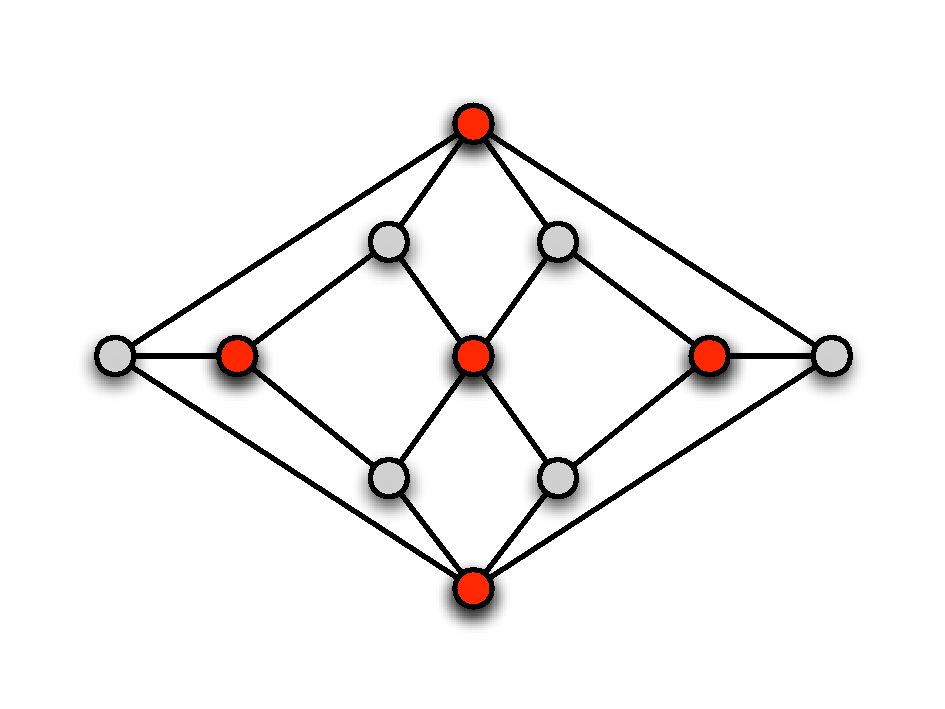
\includegraphics[width=0.6\textwidth]{pic1.pdf}
\end{center}
\caption{Herschelov graf, vektorska grafika.}
\label{pic1}
\end{figure}
Pa res lahko vključimo slike katerihkoli formatov? 
Žal ne. 
Programski paket \LaTeX\ lahko uporabljamo v več dialektih. 
Ukaz {\tt latex} ne mara vključenih slik v formatu Portable Document Format {\tt .pdf}, ukaz {\tt pdflatex} pa ne prebavi slik v Encapsulated Postscript Formatu {\tt .eps}.
Strnjeno je vključevanje različnih vrst slikovnih datotek prikazano v tabeli~\ref{tbl:1}.

\begin{table}
\begin{center}
\begin{tabular}{l|ccc}
ukaz/format & {\tt .pdf} & {\tt .eps} & ostali formati \\ \hline
{\tt pdflatex} & da & ne & da \\
{\tt latex}   & ne & da  & da
\end{tabular}
\end{center}
\caption{Kompatibilnost različnih formatov slikovnih datotek z različnimi dialekti  \LaTeX a.}
\label{tbl:1}
\end{table}

Nasvet? 
Odločite se za uporabo ukaza {\tt pdflatex}. Vaš izdelek bo brez vmesnih stopenj na voljo v {.pdf} formatu in ga lahko odnesete v vsako tiskarno. 
Če morate na vsak način vključiti sliko, ki jo imate v {\tt .eps} formatu, jo vnaprej pretvorite v alternativni format, denimo {\tt .pdf}.

Včasih se da v okolju za uporabo programskega paketa \LaTeX\ nastaviti na kakšen način bomo prebavljali vhodne dokumente. 
Spustni meni na Sliki~\ref{pic2} odkriva uporabo \LaTeX{}a v njegovi pdf inkarnaciji --- {\tt pdflatex}.
\begin{figure}[t]
\begin{center}

\includegraphics[width=10cm]{pic2.png}
\end{center}
\caption{Kateri dialekt uporabljati?}
\label{pic2}
\end{figure}
Vključena slika~\ref{pic2} je seveda bitna.

Na vse tabele se moramo v besedilu, podobno kot na slike, tudi sklicevati, saj kot plovke v oblikovanem besedilo niso nujno na istem mestu kot v izvornem besedilu.


\subsection{Podnapisi k slikam in tabelam}

Vsaki sliki ali tabeli moramo dodati podnapis, ki na kratko pojasnuje, kaj je na sliki ali tabeli. 
Če nekdo le prelista diplomsko delo, naj bi že iz slik in njihovih podnapisov lahko na grobo razbral, kakšno temo naloga obravnava.

Če slike povzamemo iz drugih virov, potem se moramo v podnapisu k taki sliki sklicevati na ta vir!


\chapter{Struktura strokovnih besedil}
\label{stroka}

Strokovna besedila imajo ustaljeno strukturo, da bi lahko hitreje in lažje brali in predvsem razumeli taka besedila, saj načeloma vemo vnaprej, 
kje v besedilu se naj bi nahajale določene informacije.

Najbolj osnovna struktura strokovnega besedila je:
\begin{description}
\item[naslov besedila,] ki naj bo sicer kratek, a kljub temu dovolj poveden o vsebini besedila,
\item[imena avtorjev] so običajno navedena po teži prispevka, prvi avtor je tisti, ki je besedilo dejansko pisal, zadnji pa tisti, ki je raziskavo vodil,
\item[kontaktni podatki] -- poleg imena in naslova institucije je potreben vsaj naslov elektronske pošte,
\item[povzetek] je kratko besedilo, ki povsem samostojno povzame vsebino in izpostavi predvsem  glavne rezultate ali zaključke,
\item[ključne besede] so tudi namenjene iskanju vsebin med množico člankov,
\item[uvodno poglavje] uvede bralca v tematiko besedila, razloži kaj je namen besedila, predstavi področje o katerem besedilo piše 
(če temu ni namenjeno v celoti posebno poglavje) ter na kratko predstavi strukturo celotnega besedila,
\item[poglavja] tvorijo zaokrožene celote, ki se po potrebi še nadalje členijo na podpoglavja, namenjena so recimo opisu orodij, 
ki smo jih uporabili pri delu, teoretičnim rezultatom ali predstavitvi rezultatov, ki smo jih dosegli,
\item[zaključek] še enkrat izpostavi glavne rezultate ali ugotovitve, jih primerja z dosedanjimi in morebiti poda tudi ideje za nadaljne delo,
\item[literatura] je seznam vseh virov, na katere smo se pri svojem delu opirali, oziroma smo se na njih sklicevali v svojem besedilu.
\end{description}

Naslove poglavij in podpoglavij izbiramo tako, da lahko bralec že pri prelistavanju diplome in branju naslovov
v grobem ugotovi, kaj je vsebina diplomskega dela.

Strokovna besedila običajno pišemo v prvi osebi množine, v nevtralnem in umirjenem tonu. 
Uporaba sopomenk ni zaželjena, saj želimo zaradi lažjega razumevanja za iste pojme vseskozi uporabljati iste besede.
Najpomenbnejše ugotovitve je smiselno večkrat zapisati, na primer v povzetku, uvodu, glavnem delu in zaključku.
Vse trditve naj bi temeljile bodisi na lastnih ugotovitvah (izpeljavah, preizkusih, testiranjih) ali pa z navajanjem ustreznih virov.

Največ se lahko naučimo s skrbnim branjem dobrih zgledov takih besedil.


\chapter{Pogoste napake pri pisanju v slovenščini}  % poglavje dodal Solina
\label{slo}

V slovenščini moramo paziti  pri uporabi pridevnikov, ki se ne sklanjajo kot so npr. kratice. 
Pravilno pišemo model CAD in \textbf{ne} CAD model!

Pri sklanjanju tujih imen ne uporabljamo vezajev, pravilno je Applov operacijski sistem in \textbf{ne} Apple-ov.

Pika, klicaj in vprašaj so levostični: pred njimi ni presledka, za njimi pa. 
Klicajev in vprašajev se v strokovnih besedilih načeloma izogibamo. Oklepaji so desnostični in zaklepaji levostični (takole).

V slovenščini pišemo narekovaje drugače kot v angleščini!   
Običajno uporabljamo dvojne spodnje-zgornje narekovaje:  \sn{slovenski narekovaji}.
Za slovenske narekovaje je v tej LaTeXovi predlogi definiran nov ukaz \verb+ \sn{ ... }+.

Vezaj  je levo in desno stičen: \verb=slovensko-angleški slovar= in ga pišemo z enim pomišljajem.

V slovenščini je pred in po pomišljaju presledek, ki ga v LaTeXu pišemo z dvema pomišljajema: \verb=Pozor -- hud pes!=
V angleščini pa je za razliko pomišljaj levo in desno stičen in se v LaTeXu piše s tremi  pomišljaji: \verb=---=.
S stičnim pomišljajem pa lahko nadomeščamo predlog od \dots do, denimo pri navajanju strani, npr. preberite strani 7--11 (\verb=7--11=).



\sn{Pred ki, ko, ker, da, če vejica skače}. To osnovnošolsko pravilo smo v življenju po potrebi uporabljali, dopolnili, morda celo pozabili. 
Pravilo sicer drži, ampak samo če je izpolnjenih kar nekaj pogojev (npr. da so ti vezniki samostojni, enobesedni, ne gre za vrivek itd.).
Povedki so med seboj ločeni z vejicami, razen če so zvezani z in, pa, ter, ne–ne, niti–niti, ali, bodisi, oziroma.
Sicer pa je bolje pisati kratke stavke kot pretirano dolge.

V računalništvu se stalno pojavljajo novi pojmi in nove besede, za katere pogosto še ne obstajajo uveljavljeni slovenski izrazi.
Kadar smo v dvomih, kateri slovenski izraz je primeren, si lahko pomagamo z Računalniškim slovarčkom~\cite{slovarcek}.





\chapter{Koristni nasveti pri pisanju v \LaTeX{u}}   % poglavje dodal Solina
\label{latex}

Programski paket \LaTeX\ je bil prvotno predstavljen v priročniku~\cite{lamport} in je v resnici nadgradnja sistema \TeX\ avtorja Donalda Knutha~\cite{knuth}, 
znanega po svojih knjigah o umetnosti programiranja, 
ter Knuth-Bendixovem algoritmu~\cite{knuth1983simple}.

Različnih implementacij \LaTeX{}a je cela vrsta.
Za OS X priporočamo TeXShop, za Windows PC pa MikTeX.
Spletna verzija, ki poenostavi sodelovanje pri pisanju, je Overleaf.

Včasih smo si pri pisanju v \LaTeX{}u  pomagali predvsem s tiskanimi pri\-ro\-čni\-ki, danes pa je enostavneje in hitreje, da ob vsakem problemu za pomoč enostavno povprašamo Google, 
saj je na spletu cela vrsta forumov za pomoč pri \TeX{}iranju.

\LaTeX\ včasih ne zna deliti slovenskih besed, ki vsebujejo črke s strešicami. 
Če taka beseda štrli preko desnega roba,  \LaTeX{}u pokažemo, kje lahko tako besedo deli, takole: \verb=ra\-ču\-nal\-ni\-štvo=.
Katere vrstice štrlijo preko desnega roba, se lahko prepričamo tako, da dokument prevedemo s vključeno opcijo \texttt{draft}: \verb=\documentclass[a4paper, 12pt, draft]{book}=.


Predlagamo, da v izvornem besedilu začenjate vsak stavek v novi vrstici, saj \LaTeX\ sam razporeja besede po vrsticah postavljenega besedila. 
Bo pa zato iskanje po izvornem besedilu in popravljanje veliko hitrejše. 
Večina sistemov za \TeX{}iranje sicer omogoča s klikanjem enostavno prestopanje  iz prevedenega besedila na ustrezno mesto v izvornem besedilu in obratno.

Boljšo preglednost dosežemo, tako kot pri pisanju programske kode, tudi z izpuščanjem praznih vrstic za boljšo preglednost strukture izvornega besedila.

S pomočjo  okolja \verb=\begin{comment} ... \end{comment}= lahko  hkrati zakomentiramo več vrstic izvornega besedila.

Pri spreminjanju in dodajanju izvornega besedila je najbolje pogosto prevajati, da se sproti prepričamo, če so naši nameni izpolnjeni pravilno.

Kadar besedilo, ki je že bilo napisano z nekim vizualnim urejevalnikom (npr. z Wordom), želimo prenesti v \LaTeX, je tudi najbolje to delati postopoma s posameznimi bloki besedila, 
tako da lahko morebitne napake hitro identificiramo in odpravimo.
Za prevajanje Wordovih datotek v \LaTeX\ sicer obstajajo prevajalniki, ki pa običajno ne generirajo tako čisto logično strukturo besedila, kot jo  \LaTeX\ omogoča.
Hiter in enostaven način prevedbe besedila, ki  zahteva sicer ročne dopolnitve, poteka tako, da besedilo urejeno z vizualnim urejevalnikom najprej shranimo v formatu pdf, 
nato pa to besedilo uvozimo v urejevalnik, kjer urejamo izvorno besedilo v formatu \LaTeX.




\section{Pisave v \LaTeX u}

V  \LaTeX ovem okolju lahko načeloma uporabljamo poljubne pisave. 
Izbira poljubne pisave pa ni tako enostavna kot v vizualnih urejevalnikih besedil.
Posamezne oblikovno medseboj usklajene pisave so običajno združene v družine pisav.
V \LaTeX u se privzeta družina pisav imenuje Computer Modern,
kjer so poleg navadnih črk (roman v \LaTeX u) na voljo tudi kurzivne črke (\textit{italic} v \LaTeX u), 
krepke (\textbf{bold} v \LaTeX u), kapitelke (\textsc{small caps} v \LaTeX u), linearne črke ({\textsf{san serif} v \LaTeX u)                                                                                                                                                                                                                                                                                                                         
in druge pisave.
V istem dokumentu zaradi skladnega izleda uporabljamo običajno le pisave ene družine. 

Ko začenjamo uporabljati \LaTeX, je zato najbolj smiselno uporabljati kar privzete pisave, s katerimi je napisan tudi ta dokument.
Z ustreznimi ukazi  lahko nato preklapljamo med navadnimi, kurzivnimi, krepkimi in drugimi pisavami. 
Zelo enostavna je tudi izbira velikosti črk.
\LaTeX\  odlično podpira večjezičnost, tudi v sklopu istega dokumenta, saj obstajajo pisave za praktično vse jezike, tudi take, ki ne uporabljajo latinskih črk.

Za prikaz programske kode se pogosto uporablja pisava, kjer imajo vse črke enako širino, kot so  črke na mehanskem pisalnem stroju ({\texttt{typewriter} v \LaTeX u).

Najbolj priročno okolje za pisanje kratkih izsekov programske kode je okolje \texttt{verbatim}, saj ta ohranja vizualno organizacijo izvornega besedila in ima privzeto pisavo pisalnega stroja.

\begin{verbatim}
for (i = 0; i < 100; i++)
   for (j = i; j < 10; j++)
      some_function(i, j);
\end{verbatim}


\chapter{Kaj pa literatura?}
\label{lit}

Kot smo omenili že v uvodu, je pravi način za citiranje literature uporaba \BibTeX{}a~\cite{bib}. 
\BibTeX\ zagotovi, da nobene obvezne informacije pri določeni vrsti literature ne izpustimo in da vse informacije o določeni vrsti vira dosledno navajamo na enak način.

Osnovna ideja \BibTeX{a} je, da vse informacije o literaturi zapisujemo v posebno datoteko, v našem primeru je to \texttt{literatura.bib}.
Vsakemu viru v tej datoteki določimo simbolično ime.
V  našem primeru je v tej datoteki nekaj najbolj značilnih zvrsti literature, kot so knjige~\cite{lamport}, 
članki v revijah~\cite{leonardo} in zbornikih konferenc~\cite{poglavje_springer}, 
spletni viri~\cite{bib,slovarcek,video}, 
tehnično poročilo~\cite{andersen2012kinect}, 
diplome~\cite{diploma} itd.
Diploma~\cite{diploma} iz leta 1990 je bila prva diploma na Fakulteti za elektrotehniko in računalništvo, ki je bila oblikovana z \LaTeX om!
Novej\v se reference, ki so spletnih straneh svojih založnikov arhivirane v elektronski obliki, imajo določeno \v stevilko DOI: \url{http://dx.doi.org}, ki jo tudi lahko vključimo v izpis literature in omogoča neposredno povezavo do te reference~\cite{Kljun2018}.

Po vsaki spremembi pri sklicu na literaturo moramo najprej prevesti izvorno besedilo s prevajalnikom \LaTeX, nato s prevajalnikom  \BibTeX, ki ustvari datoteko  {\tt vzorec\_dip\_Seminar.bbl}, in nato še dvakrat s prevajalnikom  \LaTeX.

Kako natančno se spisek literature nato izpiše (ali po vrstnem redu sklicevanja, ali po abecedi priimkov prvih avtorjev, ali se imena avtorjev pišejo pred priimki itd.) je odvisno od stilske datoteke.
V diplomi bomo uporabili osnovno stilsko datoteko \texttt{plain}, oz. \texttt{plainnat}, ki vire razporedi po abecedi.
Zato je potrebno pri določenih zvrsteh literature, ki nima avtorjev, dodati polje \texttt{key}, ki določi vrstni red vira po abecedi.

Z uporabo \BibTeX{a} v slovenščini je še nekaj nedoslednosti, saj so pomožne besede, ki jih \BibTeX\ sam doda,  kot so \textit{editor},  \textit{pages} in besedica  \textit{and} pred zadnjim avtorjem, 
če ima vir več avtorjev~\cite{andersen2012kinect}, zapisane v angleščini,
čeprav smo izbrali opcijo \texttt{slovene} pri paketu \texttt{babel}.
To nedoslednost je možno popraviti z ročnim urejanjem datoteke {\tt vzorec\_dip\_Seminar.bbl}, 
kar pa je smiselno šele potem, ko bibliografije v datoteki \texttt{literatura.bib} ne bomo več spreminjali,
oziroma ne bomo več dodajali novih sklicev na literaturo v izvornem besedilu.
Vsebino datoteke {\tt vzorec\_dip\_Seminar.bbl} lahko na koncu urejanja tudi vključimo kar v izvorno besedilo diplome, tako da je vso besedilo, vključno z literaturo, zajeto le v eni datoteki.

Ko začenjamo uporabljati \BibTeX\ je lažje, če za urejanje datoteke .bib uporabljamo kar isti urejevalnik kot za urejanje datotek .tex, 
čeprav obstajajo tudi posebni urejevalniki oziroma programi za delo z \BibTeX om.

Le če se bomo na določen vir v besedilu tudi sklicevali, se bo pojavil tudi v spisku literature.
Tako je avtomatično zagotovljeno, da se na vsak vir v seznamu literature tudi sklicujemo v besedilu diplome.
V datoteki \texttt{.bib} imamo sicer lahko veliko več virov za literaturo, kot jih bomo uporabili v diplomi.

Vire v formatu \BibTeX\ lahko enostavno poiščemo in prekopiramo iz spletnih strani založnikov ali različnih akademskih spletnih portalov za iskanje znanstvene literature v našo datoteko \texttt{.bib}.
Izvoz  referenc v Google učenjaku še dodatno poenostavimo, če v nastavitvah izberemo \BibTeX\ kot želeni format za izvoz navedb.
Navedbe, ki jih na tak način prekopiramo, pa moramo pred uporabo vseeno preveriti, saj so taki navedki pogosto generirani povsem avtomatično in lahko vsebujejo napačne ali nepopolne podatke.

Pri sklicevanju na literaturo na koncu stavka moramo paziti, da je pika po ukazu \verb=\cite{ }=.
Da \LaTeX\ ne bi delil vrstico ravno tako, da bi sklic na literaturo v oglatih oklepajih začel novo vrstico, lahko pred sklicem na literaturo dodamo nedeljiv presledek: \verb=~\cite{ }=.


\section{Izbiranje virov za spisek literature}

Dandanes  se skoraj  vsi pri iskanju informacij vedno najprej lotimo iskanja preko svetovnega spleta.
Rezultati takega iskanja pa so pogosto spletne strani, ki danes obstajajo, jutri pa jih morda ne bo več, ali pa vsaj ne v taki obliki, kot smo jo prebrali.
Smisel navajanja literature pa je, da tudi po dolgih letih nekdo, ki bo bral vašo diplomo, lahko poišče vire, ki jih navajate v diplomi.
Taki viri pa so predvsem članki v znanstvenih revijah, ki se arhivirajo v knjižnicah, založniki teh revij pa večinoma omogočajo tudi elektronski dostop do arhiva vseh njihovih člankov.

Znanstveni rezultati, ki so objavljeni v obliki recenziranih člankov, bodisi v konferenčnih zbornikih, še bolje pa v znanstvenih revijah, so veliko bolj izčiščen in zanesljiv vir informacij, saj
so taki članki šli skozi recenzijski postopek.
Zato na svetovnem spletu začenjamo iskati vire za strokovna besedila predvsem preko akademskih spletnih portalov, kot so npr. Google učenjak, Research Gate ali Academia, saj
so na teh portalih rezultati iskanja le akademske publikacije.
Če je za dostop do nekega članka potrebno plačati, se obrnemo za pomoč in dodatne informacije na  našo knjižnico.

Če res ne gre drugače, pa je pomembno, da pri sklicevanju na spletni vir, vedno navedemo tudi datum, kdaj smo dostopali do tega vira.



\chapter{Sistem STUDIS in PDF/A}
\label{PDF}

Elektronsko verzijo diplome moramo oddati preko sistema STUDIS v formatu PDF/A ~\cite{pdfa}.
Natančneje v formatu PDF/A-1b. 

\LaTeX\ in omenjeni format imata še nekaj težav s sobivanjem. 
Paket \texttt{pdfx.sty}, ki naj bi \LaTeX{u} omogočal podporo formatu PDF/A ne deluje v skladu s pričakovanji. 
Ta predloga delno ustreza formatu, vsekakor dovolj, da jo študentski informacijski sistem sprejme. 
Znaten del rešitve je prispeval Damjan Cvetan.

V predlogi, poleg izvornega  dokumenta \texttt{.tex} in vloženih slik \texttt{pic1.pdf} in \texttt{pic2.png}, 
potrebujemo še predlogo datoteke z metapodatki \texttt{pdfa-1b.xmp} in datoteko z barvnim profilom \texttt{sRGBIEC1966-2.1.icm}.




\chapter{Sklepne ugotovitve}

Uporaba \LaTeX{a} in \BibTeX{a} je v okviru Diplomskega seminarja \textbf{obvezna}!
Izbira \LaTeX\ ali ne \LaTeX\ pri pisanju dejanske diplomske naloge pa je pre\-pu\-šče\-na dogovoru med vami in vašim mentorjem.

Res je, da so prvi koraki v \LaTeX{}u težavni. 
Ta dokument naj vam služi kot začetna opora pri hoji.
Pri kakršnihkoli nadaljnih vprašanjih ali napakah pa svetujem uporabo Googla, saj je spletnih strani za pomoč pri odpravljanju težav pri uporabi \LaTeX{}a ogromno.

Preden diplomo oddate na sistemu STUDIS, še enkrat preverite, če so slovenske besede, ki vsebujejo črke s strešicami,  pravilno deljene.
Poravnavo po vrsticah pa kontrolirajte tako, da izvorno datoteko prevedete z opcijo \texttt{draft}, kar vam pokaže predolge vrstice.


\cleardoublepage
\addcontentsline{toc}{chapter}{Literatura}
\bibliography{literatura}
\bibliographystyle{plainnat}

\end{document}

